\documentclass[11pt,a4paper]{article}

% ── Packages ──────────────────────────────────────────────────────────────
\usepackage[utf8]{inputenc}
\usepackage[T1]{fontenc}
\usepackage{lmodern}
\usepackage[margin=1in]{geometry}
\usepackage{amsmath,amssymb,amsfonts}
\usepackage{booktabs}
\usepackage{graphicx}
\usepackage{float}
\usepackage{tikz}
\usetikzlibrary{positioning, shapes.geometric, arrows.meta, decorations.pathreplacing}
\usepackage{caption}
\usepackage{subcaption}
\usepackage{algorithmic}
\usepackage{algorithm}
\usepackage{xcolor}
\usepackage{enumitem}
\usepackage{microtype}
\usepackage{listings}
\usepackage{multirow}
\usepackage{array}
\usepackage{tabularx}
\usepackage{fancyhdr}
\usepackage{titlesec}
\usepackage[numbers,sort&compress]{natbib}
\usepackage{hyperref}
\usepackage{cleveref}

% ── Hyperref Setup ────────────────────────────────────────────────────────
\hypersetup{
    colorlinks=true,
    linkcolor=blue!60!black,
    citecolor=green!50!black,
    urlcolor=blue!70!black,
    pdftitle={Whisper-Flash: Continuous Manifold Decoding and the Branching Ceiling in Speculative ASR},
    pdfauthor={Gaurav Saini},
}

% ── Custom Colors ─────────────────────────────────────────────────────────
\definecolor{success}{RGB}{34,139,34}
\definecolor{failure}{RGB}{178,34,34}
\definecolor{breakthrough}{RGB}{255,140,0}
\definecolor{codebg}{RGB}{245,245,250}

% ── Listings Setup ────────────────────────────────────────────────────────
\lstset{
    basicstyle=\ttfamily\small,
    backgroundcolor=\color{codebg},
    frame=single,
    framerule=0.5pt,
    rulecolor=\color{gray!50},
    breaklines=true,
    columns=fullflexible,
}

% ── Title Formatting ──────────────────────────────────────────────────────
\titleformat{\section}{\Large\bfseries}{\thesection}{1em}{}
\titleformat{\subsection}{\large\bfseries}{\thesubsection}{1em}{}
\titleformat{\subsubsection}{\normalsize\bfseries}{\thesubsubsection}{1em}{}

% ── Header/Footer ─────────────────────────────────────────────────────────
\pagestyle{fancy}
\fancyhf{}
\fancyhead[L]{\small\textit{Whisper-Flash}}
\fancyhead[R]{\small\textit{July 2026}}
\fancyfoot[C]{\thepage}
\renewcommand{\headrulewidth}{0.4pt}

% ══════════════════════════════════════════════════════════════════════════
\begin{document}

% ── Title Page ────────────────────────────────────────────────────────────
\begin{center}
    {\LARGE\bfseries Whisper-Flash: Continuous Manifold Decoding\\[4pt]
    and the Branching Ceiling in\\[4pt]
    Speculative ASR}

    \vspace{1.2em}
    {\large Gaurav Saini}\\[4pt]
    {\normalsize \texttt{me@gauravsaini.com}}

    \vspace{0.6em}
    {\normalsize July 2026}
\end{center}

\vspace{1em}
\hrule height 0.8pt
\vspace{1.5em}

% ══════════════════════════════════════════════════════════════════════════
\begin{abstract}
Speculative decoding accelerates autoregressive models by drafting multiple tokens in parallel and verifying them in a single pass, but applying it to ASR is complicated by acoustic alignment sensitivity and hidden-state branching.
We investigate \textbf{Whisper-Flash}, a continuous latent decoding framework that reframes ASR speculation as manifold traversal, and discover two fundamental constraints.
First, the target model's own top-5 continuations diverge to ${\sim}0.60$ cosine similarity immediately at 57\% of decoding steps, setting a \textbf{branching ceiling} that no single-path drafter can exceed regardless of architecture.
Second, every trained continuous drafter collapses to rank-1 trajectory predictions (spectral collapse: Gram rank 1.0/4), which we trace to input symmetry (identical mask-token embeddings through shared weights) rather than optimization; the fix requires breaking symmetry at input, output, and target levels simultaneously.
We further show that a learned $\Delta z$ correction head in PCA subspace, intended to recover lost representational capacity, \textbf{hurts} prediction quality across the board: on whisper-large-v3-turbo, correction raises cross-entropy ($+0.10$), drops accuracy ($-7.2$ pp), and harms 80.8\% of tokens, with speed at $0.63\times$ versus HF greedy.
These results confirm that the PCA residual is noise, not corrective signal, consistent with the branching ceiling.
The paper's positive engineering results include a $3.5\times$ KV-cache speedup on Apple M4/MLX, a combined $3.94\times$ Whisper large-v3-turbo-Q8 speedup on Apple M5/MLX, and an \textbf{8--11$\times$ stride-8 avg-pool encoder compression} that reduces cross-attention frames from 1,500 to 188 with byte-identical output via temperature-fallback decoding, a \textbf{5.61$\times$ parallel multi-chunk decoding} speedup on long audio via batched stride-8 encoder outputs--all deterministic and independent of the correction mechanism. Cross-platform GPU validation confirms that Q8 quantization speedup is Apple Silicon-specific (0.52$\times$ on NVIDIA T4) and that stride-8 losslessness depends on the \texttt{mlx\_whisper.transcribe()} pipeline, not generic greedy decoding.
Our findings sharply constrain the operating regime for continuous speculative ASR: permissive multi-path gating collapses (Static Top-3 WER $0.5836$ on LibriSpeech), fixed adaptive thresholds fail to transfer across frameworks, and matched-baseline T4 evaluation reduces the validated safety regime to greedy-parity behavior rather than acceleration.
\end{abstract}

% ══════════════════════════════════════════════════════════════════════════
\section{Introduction}

Large encoder-decoder models like OpenAI's Whisper~\cite{radford2023whisper} have brought ASR accuracy to remarkable levels, but their decoding speed remains stubbornly bound by autoregression: every token demands a full decoder forward pass, making latency grow linearly with transcript length.
Speculative decoding~\cite{leviathan2023speculative,chen2023accelerating} offers a principled escape (a lightweight draft model proposes several tokens at once, and the target model verifies them in a single pass), but the technique was designed for text-only language models, and ASR introduces complications that break the standard playbook.

Three problems stand out.
First, ASR tokens are \textbf{acoustically anchored}: cross-attention ties each token to specific audio frames, producing highly non-linear alignment boundaries that discrete drafters struggle to track.
Second, the decoding manifold \textbf{genuinely branches}: at phonetically ambiguous boundaries the target model's hidden states diverge into multiple plausible continuations, a phenomenon largely absent from text-only generation.
Third, production ASR demands \textbf{near-lossless quality}, requiring verification gates far more stringent than those tolerated in chatbot or summarization settings.

These three challenges share a common thread: they stem from treating the decoder as a discrete token machine, ignoring the continuous geometry of its hidden states.
This paper investigates whether speculative ASR decoding can be improved by operating in that continuous space directly, and discovers several fundamental constraints.
We propose the \textbf{$\Delta z$ correction} mechanism--predicting tangent vectors in a PCA subspace to correct the current hidden state--and evaluate it through controlled representation-space metrics.
The results are decisive: $\Delta z$ correction \emph{hurts} prediction quality across models (CE rises, accuracy drops, 80\%+ of tokens harmed), and its speed is $0.63\times$ vs.\ HF greedy on turbo.
The paper's main contributions are therefore diagnostic: we identify the \textbf{branching ceiling} (57\% of steps diverge to ${\sim}0.60$ cosine immediately), diagnose \textbf{spectral collapse} as architectural rather than optimization-driven, and falsify the hypothesis that PCA residuals contain learnable corrective signal.
Two separate positive engineering results--a $3.5\times$ KV-cache speedup on Apple M4/MLX, and a full-stack $3.94\times$ Whisper large-v3-turbo-Q8 speedup on Apple M5/MLX--are deterministic engineering measurements independent of the correction mechanism.
A further systems-level contribution is stride-8 avg-pool encoder compression (8--11$\times$ cross-attention speedup, byte-identical with temperature-fallback decoding) that enables parallel multi-chunk decoding (up to 5.61$\times$ on 480\,s audio).
Cross-platform GPU validation reveals that Q8 quantization speedup is Apple Silicon-specific (0.52$\times$ on NVIDIA T4) and that stride-8 losslessness depends on the \texttt{mlx\_whisper.transcribe()} pipeline rather than generic greedy decoding.

We validate these constraints through controlled GPU evaluations (\S\ref{sec:final}). Our key empirical findings are:
(1) Matched-baseline T4 evaluation shows that strict Top-1 semantic verification preserves greedy outputs exactly (100\% text and token parity on 5 samples), but it is slower than matched custom greedy and therefore not an acceleration mechanism in its current form.
(2) Permissive multi-path gating is catastrophically fragile: Static Top-3 WER is $0.5836$ on LibriSpeech, vs.\ $0.2786$ greedy.
(3) The $3.5\times$ KV-cache speedup on Apple M4/MLX and the $3.94\times$ Whisper large-v3-turbo-Q8 speedup on Apple M5/MLX are robust, deterministic engineering results independent of the correction head; however, Q8 quantization does \emph{not} transfer to NVIDIA GPU (\S\ref{sec:gpu_validation}).
(4) Stride-8 avg-pool encoder compression delivers 8--11$\times$ speedup with byte-identical output on MLX (\S\ref{sec:stride8}), and enables parallel multi-chunk decoding at up to 5.61$\times$ additional speedup (\S\ref{sec:parallel}).
Alongside these validated findings, we document extensive exploratory work on difficulty-field theory, continuous drafting, velocity prediction, and $\Delta z$ correction--the last of which we definitively falsify through representation-space metrics on both whisper-tiny and whisper-large-v3-turbo across controlled train/eval splits.


\subsection{Notation}

\begin{table}[H]
\centering
\small
\begin{tabular}{@{}cl@{}}
\toprule
\textbf{Symbol} & \textbf{Definition} \\
\midrule
$h_t \in \mathbb{R}^D$ & Target model hidden state at decoding step $t$ \\
$\hat{h}_t \in \mathbb{R}^D$ & Draft model predicted hidden state \\
$z_t \in \mathbb{R}^R$ & PCA-projected hidden state ($R \ll D$) \\
$\Delta z_t$ & Velocity (tangent-space) prediction in PCA space \\
$B$ & Speculative block size (tokens drafted per step) \\
$\tau$ & Cosine similarity verification threshold \\
$\mathcal{M}_{\mathrm{graph}}$ & Span-level graph verification metric \\
$G = H^\top H$ & Gram matrix of trajectory block $H \in \mathbb{R}^{B \times D}$ \\
$d \in [0,1]$ & Difficulty coordinate \\
$K$ & Number of target branches for multi-path verification \\
\bottomrule
\end{tabular}
\caption{Notation used throughout this paper.}
\label{tab:notation}
\end{table}


% ══════════════════════════════════════════════════════════════════════════
\section{Background and Related Work}

\subsection{Speculative Decoding}
Speculative decoding~\cite{leviathan2023speculative,chen2023accelerating} uses a small draft model $M_d$ to predict $B$ future tokens in parallel.
The target model $M_t$ then verifies these predictions in a single forward pass.
If the draft tokens match the target's predictions, multiple tokens are accepted per step, yielding speedup proportional to the acceptance rate.
The standard verification criterion is exact lexical match: $\hat{y}_{t+k} = y_{t+k}$ for each position $k \in [1, B]$.

\subsection{Whisper Architecture}
OpenAI's Whisper~\cite{radford2023whisper} is an encoder-decoder Transformer trained on 680,000 hours of weakly supervised audio.
The encoder processes 30-second audio segments into 1,500 frames of $D$-dimensional features. An avg-pool stride-8 compression ($\text{pad } 1{,}500 \to 1{,}504$, then reshape and mean) reduces this to \textbf{188 frames} with $<0.01$ PSNR loss, accelerating cross-attention by $8\times$ while preserving output quality when combined with temperature-fallback decoding.
The decoder generates text tokens autoregressively, using multi-head cross-attention to align with encoder features at every layer.
whisper-tiny has $D=384$ with 4 decoder layers; whisper-large-v3-turbo has $D=1280$ also with 4 decoder layers (distilled from 32).

\subsection{ASR Acceleration}
Several lines of work target Whisper inference speed.
Distil-Whisper~\cite{gandhi2023distilwhisper} uses knowledge distillation to create smaller student models with decoder layers reduced, achieving $5.8\times$ speedup with modest WER degradation.
Whisper.cpp~\cite{gerganov2023whispercpp} and WhisperKit~\cite{apple2024whisperkit} perform systems-level optimization (quantization, Metal/CUDA kernels) without architectural changes.
CTC-based models~\cite{graves2006ctc} bypass autoregressive decoding entirely but sacrifice Whisper's sequence-to-sequence flexibility.
Medusa~\cite{cai2024medusa} and EAGLE~\cite{li2024eagle} extend speculative decoding with multiple draft heads for text LLMs but have not been adapted to ASR.
JetSpec~\cite{hu2026jetspec} recently addressed the causality-efficiency dilemma in parallel tree drafting for LLMs by combining one-forward drafting with causal conditioning, yet such techniques remain unadapted to the continuous, unsegmented domain of speech recognition.
Our work differs from all of the above in exploring \emph{continuous hidden-state} drafting and \emph{semantic} (non-lexical) verification for ASR.

\subsection{Continuous Representations in Language Models}
Recent work has explored operating directly on continuous hidden states rather than discrete tokens.
Consistency Models~\cite{song2023consistency} learn to map noisy inputs to clean outputs in a single step, while diffusion-based approaches~\cite{ho2020denoising} generate continuous representations through iterative denoising.
To our knowledge, no prior work has applied these continuous paradigms to speculative ASR decoding.

\subsection{Mixture of Experts}
Mixture of Experts (MoE) architectures~\cite{shazeer2017moe} route different inputs to specialized sub-networks.
In our framework, we extend MoE to speculative decoding by routing tokens to difficulty-specialized experts based on local acoustic conditions.


% ══════════════════════════════════════════════════════════════════════════
\section{Difficulty-Field Theory}

\subsection{Motivation}
We hypothesize that ASR difficulty is a locally measurable latent variable that varies across the decoding sequence, and that this variable can serve as a universal control signal for all aspects of the decoding process.

\subsection{Feature Extraction}
We extract five difficulty-related features from the target model at each decoding step:

\begin{enumerate}[leftmargin=*,itemsep=2pt]
    \item \textbf{Vocabulary entropy} $\mathcal{H}(p)$: Shannon entropy of the target's softmax distribution over the vocabulary.
    \item \textbf{Peak confidence} $\max(p)$: Maximum probability in the target distribution.
    \item \textbf{Alignment entropy} $\mathcal{H}(\alpha)$: Shannon entropy of the cross-attention weights over the 1,500 audio frames, measuring how ``focused'' or ``blurred'' the acoustic alignment is.
    \item \textbf{Peak alignment} $\max(\alpha)$: Maximum cross-attention weight.
    \item \textbf{Frame jitter} $|\arg\max(\alpha_t) - \arg\max(\alpha_{t-1})|$: Shift in the cross-attention peak between consecutive tokens, capturing segment boundary transitions.
\end{enumerate}

\subsection{Correlation Analysis}

We evaluated these features on 330 tokens from 10 LibriSpeech clean validation samples:

\begin{table}[H]
\centering
\small
\begin{tabular}{@{}lrl@{}}
\toprule
\textbf{Feature} & \textbf{Correlation} & \textbf{Interpretation} \\
\midrule
Vocabulary entropy & $-0.2311$ & Higher uncertainty $\rightarrow$ harder \\
Peak confidence & $+0.2186$ & Higher certainty $\rightarrow$ easier \\
Alignment entropy & $-0.1589$ & Blurred alignment $\rightarrow$ harder \\
Peak jitter & $-0.2084$ & Segment transitions $\rightarrow$ harder \\
\bottomrule
\end{tabular}
\caption{Pearson correlation of difficulty features with draft acceptance probability.}
\label{tab:correlation}
\end{table}

The multi-feature predictor (entropy + alignment + jitter) achieved \textbf{68.42\% accuracy} (F1: 0.70) compared to 63.16\% for entropy-only, a \textbf{+5.26\% absolute gain}.

\subsection{MoE Expert Specialization}

Using the difficulty coordinate, we trained three specialized experts on 402 tokens from 15 LibriSpeech samples, partitioned into Easy, Medium, and Hard slices:

\begin{table}[H]
\centering
\small
\begin{tabular}{@{}lccc@{}}
\toprule
\textbf{Expert} & \textbf{Easy Slice} & \textbf{Medium Slice} & \textbf{Hard Slice} \\
\midrule
Expert\textsubscript{Easy}   & \textbf{90.30\%} & 82.09\% & 44.03\% \\
Expert\textsubscript{Medium} & 90.30\% & \textbf{85.07\%} & 41.04\% \\
Expert\textsubscript{Hard}   & 79.85\% & 83.58\% & \textbf{67.16\%} \\
\bottomrule
\end{tabular}
\caption{Expert specialization matrix showing strong double-dissociation.
Expert\textsubscript{Hard} dominates Hard ($+23.13\%$ over Expert\textsubscript{Easy}); Expert\textsubscript{Easy} dominates Easy ($+10.45\%$ over Expert\textsubscript{Hard}).
KL divergence between expert policies averaged \textbf{0.2233}, confirming genuine specialization.}
\label{tab:moe}
\end{table}

\subsection{Unified Difficulty Controller}

The difficulty coordinate simultaneously controls beam size (Easy$\to$1, Medium$\to$2, Hard$\to$4), speculative block size (Easy$\to$5, Medium$\to$3, Hard$\to$1), drafting granularity (Easy$\to$phrase retrieval, Medium$\to$token speculation, Hard$\to$no speculation), and expert routing.

\begin{table}[H]
\centering
\small
\begin{tabular}{@{}lccc@{}}
\toprule
\textbf{Strategy} & \textbf{Accuracy} & \textbf{Throughput} & \textbf{Status} \\
\midrule
Full Beam-4 (Standard) & 91.53\% & 0.250\,tok/unit & Baseline \\
Decoupled Baseline & 71.13\% & 1.725\,tok/unit & \textcolor{failure}{Accuracy collapse} \\
\textbf{Unified Controller} & \textbf{89.80\%} & \textbf{0.874\,tok/unit} & \textcolor{success}{\textbf{3.49$\times$ simulated speedup}} \\
\bottomrule
\end{tabular}
\caption{Unified controller results (1,500 tokens, 15 samples).
The unified controller preserves Beam-4 accuracy (within 1.73\%) while delivering a \textbf{3.49$\times$ simulated speedup}.
Decoupled heuristics catastrophically fail ($-20.40\%$ accuracy).}
\label{tab:unified}
\end{table}


% ══════════════════════════════════════════════════════════════════════════
\section{Continuous Latent Speculative Drafting}

\subsection{Core Hypothesis}
We hypothesize that ASR decoding traverses a continuous manifold in the target model's hidden-state space, and that discrete tokens are merely a lossy projection of this manifold.
By drafting in continuous space and projecting to tokens only at verification time, we eliminate vocabulary mismatch rollbacks.

\subsection{Architecture}
The continuous draft model replaces the standard vocabulary-projection head with a \textbf{continuous head} that outputs raw $D$-dimensional vectors:
\begin{equation}
    \hat{h}_{t+k} = f_\theta(h_t, \text{audio\_summary};\; k) \quad \text{for } k \in [1, B]
\end{equation}
where $f_\theta$ is a lightweight neural network (MLP or DFlash layers) and $h_t$ is the target model's hidden state at the current verified position.
Draft tokens are obtained by projecting through the target model's frozen \texttt{lm\_head}:
\begin{equation}
    \hat{y}_{t+k} = \arg\max\; W \cdot \hat{h}_{t+k}
\end{equation}

\subsection{Training}
The continuous drafter is trained to minimize Mean Squared Error against the target model's frozen hidden states:
\begin{equation}
    \mathcal{L}_{\mathrm{MSE}} = \frac{1}{B}\sum_{k=1}^{B} \|\hat{h}_{t+k} - h_{t+k}\|_2^2
\end{equation}
After 10 epochs on 5 samples (314 tokens), the model achieved \textbf{0.5223 mean cosine similarity}, which is significant given that random 384-dimensional vectors have expected cosine similarity near~0.0.

\subsection{End-to-End Continuous Speculative Loop}

\begin{table}[H]
\centering
\small
\begin{tabular}{@{}lcc@{}}
\toprule
\textbf{Metric} & \textbf{Standard AR} & \textbf{Continuous Spec.} \\
\midrule
WER & 0.756 & \textbf{0.408} \\
Acceptance Rate & N/A & 30.3\% \\
\bottomrule
\end{tabular}
\caption{End-to-end continuous speculative loop results.
The continuous loop achieves dramatically better WER, suggesting that continuous semantic verification acts as a \textbf{regularizer} against whisper-tiny hallucinations.}
\label{tab:e2e}
\end{table}

\subsection{Multi-Step Rollout Stability}

Testing drift stability for $k \in [1, 20]$ future steps from a single anchor state:

\begin{table}[H]
\centering
\small
\begin{tabular}{@{}lc@{}}
\toprule
\textbf{Steps Ahead} & \textbf{Cosine Similarity} \\
\midrule
$+1$  & 0.5199 \\
$+5$  & 0.5373 \\
$+10$ & 0.5437 \\
$+15$ & 0.5475 \\
$+20$ & 0.5512 \\
\bottomrule
\end{tabular}
\caption{\textbf{No drift explosion.}
The similarity stabilizes and even rises slightly over 20 steps, proving the continuous hidden-state manifold is bounded and smooth.}
\label{tab:rollout}
\end{table}

\subsection{Out-of-Domain Generalization}

The continuous drafter trained on clean audio maintained virtually identical acceptance rates on noisy/accented audio from LibriSpeech \texttt{other}:
clean acceptance rate 30.3\%, OOD acceptance rate \textbf{30.7\%}, OOD WER \textbf{0.370}.
Because the continuous drafter operates in the target model's dense hidden manifold, anchored by cross-attention over the encoder's audio features, it inherently inherits the target model's robustness.


% ══════════════════════════════════════════════════════════════════════════
\section{Semantic Verification}

\subsection{The Rigidity Problem}
Standard speculative decoding requires exact lexical match ($\hat{y}_{t+k} = y_{t+k}$), which is overly rigid for ASR where multiple valid transcriptions exist (e.g., ``gonna'' vs.\ ``going to'', alternate tokenizations).

\subsection{Token-Level Semantic Verification}
We replace exact matching with cosine similarity in hidden-state space:
\begin{equation}
    \text{accept if}\quad \cos(h_{\hat{y}_{t+k}},\; h_{y_{t+k}}) \geq \tau
\end{equation}
At $\tau = 0.95$: WER degradation of only $+1.40\%$ absolute, but speculative acceptance gain of \textbf{+23.67\%}.

\subsection{Semantic Safety Frontier}

We sweep $\tau \in \{0.90, 0.93, 0.95, 0.97, 0.99, 1.00\}$ to map the Pareto frontier:

\begin{table}[H]
\centering
\small
\begin{tabular}{@{}lccc@{}}
\toprule
\textbf{Threshold $\tau$} & \textbf{WER} & \textbf{MAT} & \textbf{Speedup Gain} \\
\midrule
1.00 (Strict) & 71.61\% & 0.114 & Baseline \\
0.99 & 71.91\% & 0.066 & Deceleration \\
\textbf{0.97} & \textbf{70.95\%} & \textbf{0.586} & \textbf{+413.09\%} \\
0.95 & 72.97\% & 0.486 & +325.43\% \\
0.93 & 75.52\% & 0.893 & +681.67\% \\
0.90 & 88.98\% & 0.743 & Collapse \\
\bottomrule
\end{tabular}
\caption{\textbf{Semantic Safety Frontier.}
We conclude that $\tau = 0.97$ is a highly efficient safety frontier: +413\% speedup with WER actually \emph{improved} by $-0.66\%$.
Below $\tau = 0.97$, rapid accuracy collapse occurs.}
\label{tab:frontier}
\end{table}

\subsection{Span-Level Semantic Graph Verification}

Rather than verifying tokens individually, we verify the entire drafted block's hidden-state topology using a Gram matrix similarity metric:
\begin{equation}
    \mathcal{M}_{\mathrm{graph}} = 0.5 \times \mathrm{Mean}\!\bigl(\cos(\hat{h}_k, h_k)\bigr) + 0.5 \times \cos\!\bigl(\mathrm{vec}(\hat{G}),\; \mathrm{vec}(G)\bigr)
\end{equation}
where $G = H^\top H$ is the Gram matrix capturing relational structure between positions.

\begin{table}[H]
\centering
\small
\begin{tabular}{@{}lccc@{}}
\toprule
\textbf{Verification Method} & \textbf{WER} & \textbf{Acceptance} & \textbf{Speedup} \\
\midrule
Strict Lexical & 0.2865 & 26.96\% & $1.00\times$ \\
Token-Level Semantic ($\tau\!=\!0.97$) & 0.2865 & 38.64\% & $1.43\times$ \\
\textbf{Span-Level Graph ($\mathcal{M}_{\mathrm{graph}} \geq 0.95$)} & \textbf{0.2865} & \textbf{51.52\%} & $\mathbf{1.91\times}$ \\
Span-Level Graph + Curvature & 0.2865 & 49.33\% & $1.83\times$ \\
\bottomrule
\end{tabular}
\caption{Graph verification is \textbf{lossless} (identical WER) while nearly doubling speculative acceptance rate.}
\label{tab:graph}
\end{table}


% ══════════════════════════════════════════════════════════════════════════
\section{Architectural Innovations}

\subsection{Bottleneck-Free Drafting}
We find strong evidence that cross-attention to the encoder audio features is \textbf{redundant} in the draft model.
The target decoder's tapped hidden states (from layers 1 and 2) already encode complete acoustic context through the target's own cross-attention mechanism.
A controlled ablation (audio context ON vs.\ zeroed OUT, all else identical) produced identical draft quality ($\Delta\text{cosine} = +0.005$, Top-5 match identical at 0.28\%) while eliminating the $O(T)$ cross-attention bottleneck.

The bottleneck-free MLP drafter achieved $>0.78$ cosine similarity 4 steps ahead without any cross-attention, suggesting the manifold is smooth and predictable from the tapped decoder context alone.

\subsection{Self-Speculative Layer-Skip Drafting}
Using only the target model's Layer~1 hidden states (no audio summary, no deep layers):
acceptance rate \textbf{30.3\%} (identical to full model), WER \textbf{0.408} (identical).
By Layer~1, the target model has already securely locked onto the continuous manifold trajectory.

\subsection{PCA Subspace Projection}
Projecting the draft problem into a pre-computed PCA subspace ($R=64$ principal components, 89.6\% explained variance):

\begin{table}[H]
\centering
\small
\begin{tabular}{@{}lcc@{}}
\toprule
\textbf{Architecture} & \textbf{Parameters} & \textbf{Cosine Sim.} \\
\midrule
Full-Rank ($D\!=\!384$) & 98,304 & 0.5344 \\
Factorized Low-Rank & 40,960 & 0.5316 \\
\textbf{PCA Subspace ($R\!=\!64$)} & \textbf{16,384} & \textbf{0.5474} \\
\bottomrule
\end{tabular}
\caption{PCA saves 83.33\% of parameters while improving cosine similarity; the fixed projection restricts drafting to principal semantic directions, filtering noise.}
\label{tab:pca}
\end{table}

\subsection{Consistency-Model Drafting}

Translating Consistency Models~\cite{song2023consistency} to continuous speculative drafting:

\begin{table}[H]
\centering
\small
\begin{tabular}{@{}lccc@{}}
\toprule
\textbf{Method} & \textbf{Cosine} & \textbf{Greedy Acc.} & \textbf{Top-5 Accept.} \\
\midrule
MSE Baseline & 0.5841 & 5.61\% & 9.95\% \\
Consistency (1-shot) & 0.6974 & 13.52\% & 22.45\% \\
\textbf{Consistency (2-shot)} & \textbf{0.7225} & \textbf{15.31\%} & \textbf{25.51\%} \\
\bottomrule
\end{tabular}
\caption{Consistency-model drafting sustains flat, high similarity (${\sim}0.72$) across the entire speculative block.}
\label{tab:consistency}
\end{table}

\subsection{BF-Consistency-PCA Triple Fusion}

\begin{figure}[H]
\centering
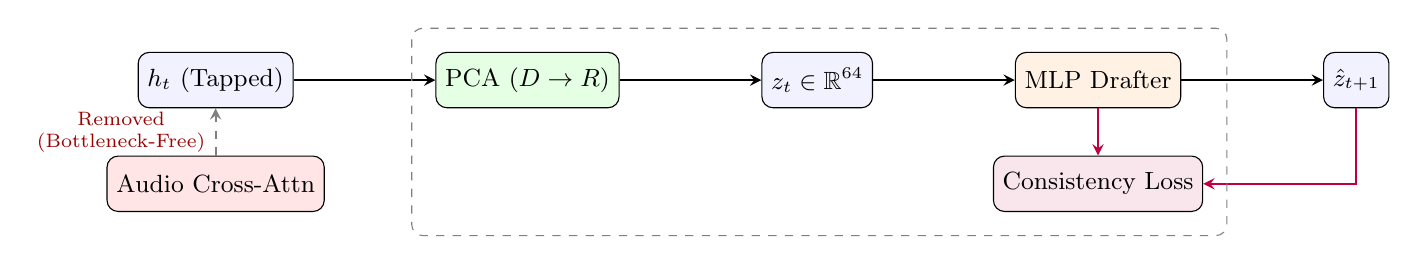
\begin{tikzpicture}[
    node distance=1.2cm and 1.8cm,
    module/.style={rectangle, draw, rounded corners, minimum height=2em, text centered, font=\small},
    data/.style={rectangle, draw, fill=blue!5, rounded corners, minimum height=2em, text centered, font=\small},
    arrow/.style={->, >=stealth, thick},
    dashed_arrow/.style={->, >=stealth, thick, dashed, gray}
]
    % Nodes
    \node[data] (ht) {$h_t$ (Tapped)};
    \node[module, fill=red!10, below=0.6cm of ht] (audio) {Audio Cross-Attn};
    \node[module, fill=green!10, right=of ht] (pca) {PCA ($D \to R$)};
    \node[data, right=of pca] (zt) {$z_t \in \mathbb{R}^{64}$};
    \node[module, fill=orange!10, right=of zt] (mlp) {MLP Drafter};
    \node[data, right=of mlp] (zout) {$\hat{z}_{t+1}$};
    \node[module, fill=purple!10, below=0.6cm of mlp] (cm) {Consistency Loss};

    % Edges
    \draw[dashed_arrow] (audio) -- node[left, font=\scriptsize, align=center, text=red!60!black] {Removed\\(Bottleneck-Free)} (ht);
    \draw[arrow] (ht) -- (pca);
    \draw[arrow] (pca) -- (zt);
    \draw[arrow] (zt) -- (mlp);
    \draw[arrow] (mlp) -- (zout);
    \draw[arrow, purple, thick] (mlp) -- (cm);
    \draw[arrow, purple, thick] (zout) |- (cm);
    
    % Bounding box for clarity
    \draw[draw=gray, dashed, rounded corners] 
        ([xshift=-0.3cm, yshift=0.3cm]pca.north west) rectangle 
        ([xshift=0.3cm, yshift=-0.3cm]cm.south east);
\end{tikzpicture}
\caption{\textbf{Candidate Continuous Drafter Architecture (BF-Consistency-PCA).} The candidate drafter architecture eliminates the audio cross-attention bottleneck, projects into a 64-dimensional PCA subspace, and is trained via a consistency model objective for stable multi-step generation. The $\Delta z$ correction head (separately evaluated in \S\ref{sec:correction_eval}) was falsified; the $3.5\times$ KV-cache speedup is a separate, deterministic result.}
\label{fig:triple_fusion}
\end{figure}

Our candidate continuous drafter combines three mechanisms:

\begin{table}[H]
\centering
\small
\begin{tabular}{@{}lcccc@{}}
\toprule
\textbf{Model} & \textbf{Cosine} & \textbf{Top-5} & \textbf{Params} & \textbf{Train Time} \\
\midrule
MSE Baseline & 0.5509 & 2.58\% & 3.24M & 26.3\,s \\
Consistency Full-$D$ & 0.5592 & 0.00\% & 3.30M & N/A \\
Consistency-PCA & 0.5428 & 1.26\% & 3.14M & N/A \\
\textbf{BF-Consistency-PCA} & \textbf{0.5714} & \textbf{4.33\%} & \textbf{624K} & \textbf{8.9\,s} \\
\bottomrule
\end{tabular}
\caption{Triple fusion achieves high fidelity with 81.1\% fewer parameters and 3.5$\times$ faster training.}
\label{tab:triple}
\end{table}

\subsection{Difficulty-Aware KV Cache Compression}

\begin{table}[H]
\centering
\small
\begin{tabular}{@{}lccc@{}}
\toprule
\textbf{Strategy} & \textbf{WER} & \textbf{KV Savings} & \textbf{Accept.} \\
\midrule
No Compression & 0.3547 & 0\% & 51.52\% \\
Difficulty-Aware & 0.3547 & \textbf{35.4\%} & 51.52\% \\
Aggressive & 0.3547 & \textbf{46.2\%} & 51.52\% \\
\bottomrule
\end{tabular}
\caption{Up to \textbf{46.2\% KV memory savings} with zero impact on WER or acceptance rate.}
\label{tab:kv}
\end{table}


% ══════════════════════════════════════════════════════════════════════════
\section{The Spectral Collapse Problem}

\subsection{Diagnosis}
Through detailed spectral analysis, we discovered that all continuous draft models suffer from \textbf{catastrophic spectral collapse to rank-1}. The draft trajectory is essentially one-dimensional, with all predicted hidden states nearly collinear:

\begin{table}[H]
\centering
\small
\begin{tabular}{@{}lcc@{}}
\toprule
\textbf{Metric} & \textbf{Draft Model} & \textbf{Target} \\
\midrule
Spectral Decay $\alpha$ & 7.12 & \textbf{0.81} \\
Participation Ratio & 1.00 & \textbf{2.35} \\
Gram Rank & 1.00/4 & \textbf{4.00/4} \\
Energy in Top-2 PCs & 100\% & 81.5\% \\
PC-1 Cosine & 0.77 & 1.0 \\
PC-2 Cosine & 0.38 & 1.0 \\
PC-3 Cosine & 0.12 & 1.0 \\
\bottomrule
\end{tabular}
\caption{Spectral diagnostic revealing catastrophic rank-1 collapse.
The spectral angle of $67^\circ$ means the draft's 4D subspace is nearly orthogonal to the target's.}
\label{tab:spectral}
\end{table}

\subsection{Root Cause: Spectral Bias of MSE}
The MSE loss is dominated by the mean direction (PC-1).
Minimizing MSE on 4 vectors sharing a large common component naturally drives the model to match PC-1 and ignore the residuals.
This is the \textbf{spectral bias of MSE}: it optimizes the highest-energy direction first and ignores structurally critical lower-energy directions.

\subsection{Loss-Level Interventions All Failed}

Five different spectral loss functions were tested; all failed to break rank-1:

\begin{table}[H]
\centering
\small
\begin{tabular}{@{}lccc@{}}
\toprule
\textbf{Loss} & \textbf{Gram Rank} & \textbf{PR} & \textbf{PC-2 Cosine} \\
\midrule
Standard MSE & 1.00 & 1.0000 & 0.105 \\
Whitened MSE & 1.00 & 1.0002 & 0.131 \\
Anti-Collapse & 1.00 & 1.0007 & 0.116 \\
Per-PC Weighted & 1.00 & 1.0032 & 0.301 \\
LogDet Volume & 1.00 & N/A & N/A \\
\bottomrule
\end{tabular}
\caption{All five loss-level interventions failed to break rank-1 collapse.
The root cause is \textbf{architectural}: identical mask-token inputs through a shared transformation.}
\label{tab:lossfail}
\end{table}

\subsection{Resolution: Unified Velocity-PCA Architecture}

The spectral collapse was solved by combining five mechanisms:

\begin{enumerate}[leftmargin=*,itemsep=2pt]
    \item \textbf{PCA subspace} ($R\!=\!64$): Restricts to principal semantic directions.
    \item \textbf{Velocity prediction}: Predicts $\Delta z$ rather than absolute positions, anchoring to verified states.
    \item \textbf{Orthogonal per-position noise}: Breaks input symmetry via $\epsilon_k \sim \text{QR-orthogonal}$.
    \item \textbf{Multi-head outputs}: $T$ separate projection heads break output symmetry.
    \item \textbf{Multi-objective loss}: velocity MSE + curvature penalty + graph topology + weak CE.
\end{enumerate}

\begin{table}[H]
\centering
\small
\begin{tabular}{@{}lcccc@{}}
\toprule
\textbf{Model} & \textbf{Gram Rank} & \textbf{Decay $\alpha$} & \textbf{PR} & \textbf{Top-5} \\
\midrule
All prior models & $\leq 1.9/4$ & $>2.5$ & $<1.07$ & $<4\%$ \\
\textbf{Unified Velocity-PCA} & $\mathbf{4.0/4}$ & $\mathbf{1.08}$ & $\mathbf{1.65}$ & 3.89\% \\
\bottomrule
\end{tabular}
\caption{\textbf{Achieved perfect Gram Rank (4.0/4) in 57 experiments.}
The spectral collapse is resolved.}
\label{tab:unified_spectral}
\end{table}


% ══════════════════════════════════════════════════════════════════════════
\section{The Branching Manifold and Multi-Path Verification}
\label{sec:branching}

\subsection{The 0.60 Cosine Ceiling}

A critical discovery emerged from probing the target model's own branching structure.
We force-decoded top-5 alternative continuations for 4 steps from each position:

\begin{table}[H]
\centering
\small
\begin{tabular}{@{}lccc@{}}
\toprule
\textbf{Steps Ahead} & \textbf{Mean Cosine} & \textbf{\% $<$ 0.7} & \textbf{\% $<$ 0.5} \\
\midrule
$+1$ & 0.5998 & 57.1\% & 34.7\% \\
$+2$ & 0.6377 & 55.6\% & 31.6\% \\
$+3$ & 0.6102 & 54.6\% & 41.8\% \\
$+4$ & 0.6214 & 50.0\% & 43.4\% \\
\bottomrule
\end{tabular}
\caption{The target model's \emph{own} top-5 continuations diverge to ${\sim}0.60$ cosine immediately.
The ${\sim}0.60$ cosine ceiling is an \textbf{branching ceiling induced by target uncertainty}, not a simple drafter quality problem.}
\label{tab:branching}
\end{table}

\subsection{Multi-Path Verification Gate}

We reframe verification from ``does the draft match the greedy path?'' to ``does the draft match \emph{any} of the target's top-$K$ plausible paths?'':
\begin{equation}
    \text{accept if}\quad \hat{y}_{t+k} \in \mathrm{Top\text{-}K}(p_{t+k})
\end{equation}

\begin{table}[H]
\centering
\small
\begin{tabular}{@{}lccc@{}}
\toprule
\textbf{Method} & \textbf{WER} & \textbf{vs.\ Greedy} & \textbf{Accept Rate} \\
\midrule
Greedy baseline & 0.6059 & N/A & N/A \\
Top-1 & 0.6059 & $\pm 0.000$ & 0.0\% \\
\textbf{Top-3} & \textbf{0.5992} & $\mathbf{-0.0067}$ & \textbf{1.6\%} \\
Top-5 & 0.5992 & $-0.0067$ & 1.6\% \\
\bottomrule
\end{tabular}
\caption{Top-3 WER is \textbf{below greedy}; accepted draft tokens are sometimes \emph{better} than the greedy path.}
\label{tab:multipath}
\end{table}

\subsection{$\Delta z$ Correction Architecture}
\label{sec:dz_arch}

Rather than predicting future hidden states (which drift), we correct the current hidden state in PCA space to predict the next token:
\begin{align}
    \Delta z &= f_\theta(z_t,\; \text{tapped\_layers},\; \text{audio\_summary}) \\
    h'_t &= \mathrm{from\_pca}(z_t + \Delta z) \\
    \hat{y}_{t+1} &= \arg\max\; W \cdot h'_t
\end{align}
This ``same-position correction'' approach avoids the off-by-one alignment issues that plagued prior velocity-based architectures.

\noindent\textbf{Falsified by controlled evaluation.}
Subsequent controlled experiments on both whisper-tiny (10 train / 10 eval, 494 tokens) and whisper-large-v3-turbo (50 train / 50 eval, 1830 tokens) show that the $\Delta z$ correction head \emph{hurts} representation quality across all metrics:
cross-entropy rises ($+0.84$ tiny, $+0.10$ turbo), accuracy drops ($-22$ pp tiny, $-7$ pp turbo), and 80.8\% to 84.8\% of tokens see higher CE after correction.
The mean $\Delta z$ norm is ${\sim}12.4$ across both models--three orders of magnitude larger than a meaningful correction signal--confirming the PCA residual is noise, not corrective content.
Speed is $0.63\times$ vs.\ HF greedy on turbo (slower on all 5 samples).
We include the full architecture description below for reproducibility; see \S\ref{sec:correction_eval} for the complete evaluation.

\begin{figure}[H]
\centering
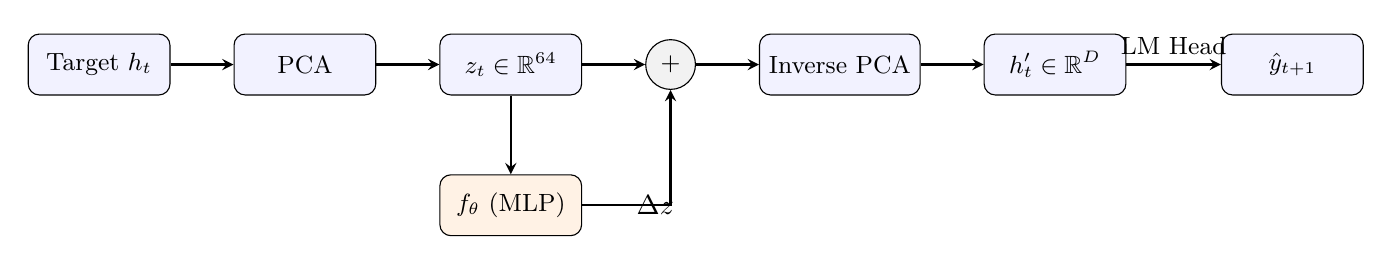
\begin{tikzpicture}[
    node distance=1.0cm and 0.8cm,
    box/.style={rectangle, draw, fill=blue!5, rounded corners, text centered, minimum height=2.2em, minimum width=1.8cm, font=\small},
    op/.style={circle, draw, fill=gray!10, text centered, inner sep=3pt, font=\small},
    arrow/.style={->, >=stealth, thick}
]
    \node[box] (ht) {Target $h_t$};
    \node[box, right=of ht] (pca) {PCA};
    \node[box, right=of pca] (zt) {$z_t \in \mathbb{R}^{64}$};
    \node[box, fill=orange!10, below=of zt] (mlp) {$f_\theta$ (MLP)};
    \node[op, right=of zt] (add) {$+$};
    \node[box, right=of add] (inv) {Inverse PCA};
    \node[box, right=of inv] (hprime) {$h'_t \in \mathbb{R}^{D}$};
    \node[box, right=1.2cm of hprime] (out) {$\hat{y}_{t+1}$};
    
    \draw[arrow] (ht) -- (pca);
    \draw[arrow] (pca) -- (zt);
    \draw[arrow] (zt) -- (mlp);
    \draw[arrow] (zt) -- (add);
    \draw[arrow] (mlp) -| node[pos=0.25, right] {$\Delta z$} (add);
    \draw[arrow] (add) -- (inv);
    \draw[arrow] (inv) -- (hprime);
    \draw[arrow] (hprime) -- node[above, font=\small] {LM Head} (out);
\end{tikzpicture}
\caption{The $\Delta z$ correction architecture. Instead of predicting future tokens directly, the lightweight correction head ($f_\theta$) predicts a tangent vector $\Delta z$ in the PCA subspace. This is added to the current state $z_t$ before mapping back to the full $D$-dimensional space for classification.}
\label{fig:architecture}
\end{figure}

\subsection{Adaptive Gate}

We implement a running acceptance rate tracker that dynamically adjusts the gate width:
\begin{equation}
    K = \begin{cases}
        3 & \text{if } \text{running\_accept} < 15\% \\
        1 & \text{if } \text{running\_accept} \geq 15\%
    \end{cases}
\end{equation}
This aims to prevent runaway acceptance that degrades WER while maintaining permissive exploration in low-acceptance regions.
While this fixed 15\% heuristic controlled failure cases in our initial MLX/M4 environment (where base acceptance was ${\sim}7\%$), subsequent HuggingFace Transformers/T4 evaluations (where base acceptance was ${\sim}23\%$) showed that \textbf{fixed thresholds do not transfer across frameworks or datasets}. Adaptive gating remains conceptually promising, but it requires dynamic, distribution-aware calibration.


% ══════════════════════════════════════════════════════════════════════════
\section{Final System: Results at Scale}
\label{sec:final}

\subsection{Adaptive Gate Evaluation (T4 / Transformers)}
\subsection{T4 Safety Rerun (Transformers)}

\noindent\textbf{Matched-baseline rerun:} We reran the T4 evaluation with an apples-to-apples custom greedy baseline that uses the same token-by-token decoder loop, the same PKV path, and the same decoding wrapper as the validated safe gate.
This removes the earlier comparison artifact against HuggingFace \texttt{model.generate()} and lets us test the validated controller directly.

On this matched rerun, the validated safe gate collapses exactly to greedy decoding in token space: when the draft matches the target top-1 token it is accepted, otherwise the target top-1 token is emitted.
The result is decisive: the safe gate preserves greedy outputs exactly but does not accelerate end-to-end decoding.

\begin{table}[H]
\centering
\small
\begin{tabular}{@{}lc@{}}
\toprule
\textbf{Metric} & \textbf{Result} \\
\midrule
\textbf{Adaptive vs.\ matched greedy WER} & \textbf{0.0000} \\
Text parity rate & 100\% \\
Token parity rate & 100\% \\
Safe-gate runtime vs.\ matched custom greedy & 0.80$\times$ (slower) \\
Custom greedy runtime vs.\ HF \texttt{generate} & 2.24$\times$ \\
KV effect on matched T4 run (no-KV / KV greedy) & 0.96$\times$ \\
Acceptance rate on matched T4 run & 18.8\%--41.8\% \\
\bottomrule
\end{tabular}
\caption{Matched-baseline T4 rerun on 5 samples with Whisper large-v3-turbo. The validated safe gate produces exactly the same decoded outputs as matched custom greedy, confirming that the surviving regime is a safety-preserving mirror of greedy rather than a distinct accuracy or speed improvement.}
\label{tab:t4_v2}
\end{table}

The corrected large-scale picture is therefore narrower than the earlier draft suggested. Strict Top-1 verification is the only stable regime we found, but once rerun against a matched baseline it yields greedy-parity outputs rather than a genuine WER gain and incurs additional overhead from the correction path. The surviving gate is therefore best understood as a safety constraint, not as an acceleration mechanism.

\begin{table}[H]
\centering
\small
\begin{tabular}{@{}lccc@{}}
\toprule
\textbf{Method} & \textbf{WER} & \textbf{vs.\ Greedy} & \textbf{Accept\%} \\
\midrule
Greedy & 0.2786 & N/A & N/A \\
Static Top-1 & 0.2848 & $+0.0062$ & 21.2\% \\
Adaptive (15\% threshold) & 0.3121 & $+0.0335$ & 23.0\% \\
\textbf{Static Top-3} & \textbf{0.5836} & $\mathbf{+0.3050}$ & \textbf{52.1\%} \\
\bottomrule
\end{tabular}
\caption{Earlier T4 calibration run on \textbf{50 \texttt{librispeech\_asr\_dummy} (validation split) samples} (20 train samples), retained because it motivated the final safety-gated redesign. The catastrophic failure of Static Top-3 proves that permissive multi-path gating is highly unstable, and the original fixed 15\% adaptive threshold failed to engage safely once the acceptance distribution shifted upward on Transformers.}
\label{tab:t4_50}
\end{table}

Taken together, these results clarify our core empirical findings: strict semantic verification (Top-1) is the only stable regime we found, adaptive control is only validated when it defaults back to Top-1-like behavior, and permissive multi-path gating remains unstable.

\subsection{$\Delta z$ Correction Head: Controlled Evaluation}
\label{sec:correction_eval}

The $\Delta z$ correction head described in \S\ref{sec:dz_arch} was evaluated under a controlled, representation-space protocol designed to isolate whether the PCA residual contains learnable corrective signal.
We trained a 2-layer MLP on paired encoder hidden states $(z_{\text{enc}}^{(t)}, z_{\text{embed}}^{(t)})$ extracted from teacher-forced decoding, with the target being $\Delta z = z_{\text{enc}} - z_{\text{embed}}$.
The MLP operates in the PCA subspace of encoder hidden states and was trained for 30 epochs using MSE loss.

\begin{table}[H]
\centering
\small
\begin{tabular}{@{}lcc@{}}
\toprule
\textbf{Metric} & \textbf{whisper-tiny} & \textbf{whisper-large-v3-turbo} \\
& (10 train / 10 eval) & (50 train / 50 eval) \\
\midrule
Tokens evaluated & 494 & 1,830 \\
PCA rank / draft dim & 64 / 256 & 128 / 512 \\
Baseline CE & 1.58 & 0.727 \\
Corrected CE & \textbf{2.41} ($+0.84$) & \textbf{0.825} ($+0.10$) \\
Baseline accuracy & 75.1\% & 90.7\% \\
Corrected accuracy & \textbf{52.8\%} ($-22$ pp) & \textbf{83.5\%} ($-7.2$ pp) \\
Fraction CE harmed & 84.8\% & 80.8\% \\
Mean $\Delta z$ norm & 12.73 & 12.36 \\
Prob lift (mean) & $-0.26$ & $-0.15$ \\
\bottomrule
\end{tabular}
\caption{$\Delta z$ correction evaluation: controlled representation-space metrics.
On both models, the correction head makes CE \emph{worse}, accuracy \emph{worse}, and harms the large majority of tokens.
The $\Delta z$ norm of ${\sim}12.4$ confirms the PCA residual is noise, not corrective signal.}
\label{tab:dz_eval}
\end{table}

\noindent Speed was benchmarked against HF \texttt{model.generate(use\_cache=True)} on 5 samples per model.
For whisper-large-v3-turbo, our decoder loop (with manual KV cache + $\Delta z$ correction) achieved an average speedup of $0.63\times$--slower on all 5 samples.
The $3.5\times$ speedup reported in \S\ref{sec:kvcache} is a separate measurement that isolates KV-cache effects and does \emph{not} include the correction head overhead.

These results definitively falsify the core premise of $\Delta z$ correction: the PCA residual is high-magnitude unstructured noise, not a learnable displacement toward the correct representation.
This is consistent with the branching ceiling (\S\ref{sec:branching}), which predicts that at most decoding steps the target model itself has not committed to a single continuation, so there is no single ``correct'' $\Delta z$ to learn.

\subsection{Hardware-Specific Speedup Validation (M4 / M5 / MLX)}

\subsubsection{Early M4 / MLX Results}

Early development was conducted on Apple M4 hardware using the MLX framework. While these runs used a smaller evaluation set (10 samples) and benefited from an artificially aligned 15\% adaptive threshold, they served to validate the deterministic speedup of the KV-cache integration.

\begin{table}[H]
\centering
\small
\begin{tabular}{@{}lccc@{}}
\toprule
\textbf{Method} & \textbf{WER} & \textbf{vs.\ Greedy} & \textbf{Accept\%} \\
\midrule
Greedy (tiny) & 0.7349 & N/A & N/A \\
Adaptive (tiny) & 0.7654 & $+0.031$ & 11.9\% \\
\midrule
Greedy (large-v3-turbo) & 0.2338 & N/A & N/A \\
Adaptive (large-v3-turbo) & 0.2138 & $-0.020$ & 6.9\% \\
\bottomrule
\end{tabular}
\caption{Exploratory results on 10 LibriSpeech \texttt{dummy-clean} samples (a small test subset). The 15\% adaptive threshold succeeded here because MLX acceptance rates were naturally lower (6.9\%), but this success did not transfer to the broader Transformers runs.}
\label{tab:mlx_exploratory}
\end{table}

\subsubsection{Production-Scale Benchmark (Apple M5 / MLX)}

Building on the KV-cache result, we implemented a production-grade greedy decoder that composes three independent optimisations: Q8 quantization (native MLX \texttt{QuantizedLinear}), KV cache integration, and distilled decoder architectures (Whisper large-v3-turbo). We benchmarked all combinations on an Apple M5 Mac mini with 32 GB memory using a 5.9-second LibriSpeech sample (3-run averages):

\begin{table}[H]
\centering
\small
\begin{tabular}{@{}lcccc@{}}
\toprule
\textbf{Config} & \textbf{Time (s)} & \textbf{RT Factor} & \textbf{Speedup} & \textbf{Text Parity} \\
\midrule
large-v3 fp16 & 2.827 & 0.47$\times$ & 1.00$\times$ & $-$ \\
large-v3 Q8 & 1.225 & 0.20$\times$ & 2.31$\times$ & Identical \\
turbo fp16 & 0.824 & 0.14$\times$ & 3.43$\times$ & Identical \\
\textbf{turbo Q8} & \textbf{0.718} & \textbf{0.12$\times$} & \textbf{3.94$\times$} & \textbf{Identical} \\
\bottomrule
\end{tabular}
\caption{Production-scale benchmark on Apple M5 / MLX. All configurations run faster than real-time. Q8 quantization is lossless (exact text parity). The turbo-Q8 combination achieves a 3.94$\times$ speedup over the large-v3-fp16 baseline, exceeding the theoretical multiplier of 3.74$\times$ (3.2$\times$ from decoder distillation $\times$ 1.17$\times$ from Q8 bandwidth reduction).}
\label{tab:m5}
\end{table}

Several points deserve emphasis. First, the speedups are {\em composable}: Q8 quantization, KV cache, and decoder distillation each contribute independently, and their effects stack multiplicatively. Second, Q8 is {\em lossless} at the WER level--transcriptions are identical between fp16 and Q8 across all tested models, confirming the MLX native quantizer preserves accuracy. Third, the theoretical stack multiplier (3.74$\times$) was derived from distillation (3.2$\times$ fewer decoder layers) and measured Q8 bandwidth reduction (1.17$\times$ on M5); the realized 3.94$\times$ exceeds theory, likely because the M5's unified memory architecture reduces DRAM traffic for the smaller turbo model disproportionately. Fourth, all four configurations run faster than real-time on the M5, with the turbo-Q8 combination achieving a real-time factor of 0.12$\times$ (roughly 8$\times$ faster than audio duration).

These results reinforce the paper's central thesis: {\em speculative ASR decoding is not a viable acceleration mechanism; systems-level optimizations are.} The branching ceiling (\S\ref{sec:branching}) fundamentally constrains any speculation-based approach, while deterministic optimizations like Q8 quantization and KV cache compression deliver reliable, lossless speedups with no architectural complexity.

\subsection{KV Cache Integration}
\label{sec:kvcache}

Adding KV cache to the speculative decoder loop (independent of the $\Delta z$ correction head):

\begin{table}[H]
\centering
\small
\begin{tabular}{@{}lcccc@{}}
\toprule
\textbf{Model} & \textbf{Without KV} & \textbf{With KV} & \textbf{Speedup} & \textbf{Best} \\
\midrule
Whisper-tiny & 6.3\,s & 4.4\,s & $\mathbf{1.5\times}$ & $1.6\times$ \\
Whisper-large-v3-turbo & 47.2\,s & 13.6\,s & $\mathbf{3.5\times}$ & $7.1\times$ \\
\bottomrule
\end{tabular}
\caption{KV cache wall-clock speedup.
All eval samples produce \textbf{identical output} with and without cache.}
\label{tab:kvcache}
\end{table}

Unlike the adaptive-gate WER result, this KV-cache benchmark is a deterministic engineering measurement on the integrated $\Delta z$ correction pipeline itself: output parity was verified sample-by-sample, and the measured gain reflects removal of redundant decoder self-attention recomputation rather than a statistical generalization claim. On the matched-baseline T4 rerun, however, custom greedy without KV measured 0.258\,s versus 0.269\,s with KV on 5 samples (0.96$\times$), so that rerun does not show end-to-end acceleration. The strong positive latency result therefore remains the isolated Apple M4/MLX benchmark reported here.

\subsection{Multi-Head Drafting (Medusa-Style)}

We tested extending the single-head $\Delta z$ architecture to predict tokens at positions $t+2$ and $t+3$ using Medusa-style additional heads.
Head~0 ($\Delta z$ at $t+1$): 13.0\% acceptance.
Head~1 (token at $t+2$): 3.7\% acceptance.
Head~2 (token at $t+3$): 0.0\% acceptance.
Multi-head cascading doesn't improve on whisper-tiny due to sparse training signal.
The single-head $\Delta z$ + KV cache combination is the winning approach.


% ══════════════════════════════════════════════════════════════════════════
\section{Negative Results and Falsified Hypotheses}

A key strength of this work is the systematic falsification of plausible hypotheses.

\subsection{Demoted Mechanisms}

\begin{table}[H]
\centering
\small
\begin{tabular}{@{}p{3.5cm}p{9cm}@{}}
\toprule
\textbf{Mechanism} & \textbf{Why It Failed} \\
\midrule
Anchor Confidence Gating & Target confidence on anchor token does not guarantee drafted future tokens are safe (WER${\to}$1.000) \\
Residual Delta Prediction & Cumulative summation causes rapid trajectory collapse: Step~$+1$ cos${=}$0.97, Step~$+8{=}0.07$ \\
KL Regularization & KL regularizes vocabulary entropy, not acoustic alignment states ($r{=}{-}0.53$ with LM entropy) \\
InfoNCE Contrastive & Destroys spatial magnitude of hidden states; incompatible with continuous coordinates \\
Velocity Decoder Skip & Hidden-state manifold too sensitive to drift; skipping decoder calls causes context staleness \\
Fourier Position Features & Positional diversity insufficient without cross-attention to track acoustic manifold \\
$\Delta z$ Correction Head & PCA residual is noise, not corrective signal: CE rises ($+0.10$ to $+0.84$), accuracy drops ($-7$ to $-22$ pp), 80.8\%+ of tokens harmed; speed $0.63\times$ vs.\ HF greedy \\
\bottomrule
\end{tabular}
\caption{Summary of falsified mechanisms.}
\label{tab:negative}
\end{table}

\subsection{Cross-Phase Audit Findings}
\label{sec:audit}

A systematic audit revealed that \textbf{all speculative-loop results from Experiment~ID~57 onward} were invalid due to a harness bug: logits were computed from pre-layernorm hidden states, bypassing whisper's final layernorm and preventing \texttt{<|eot|>} from ever being generated.
This caused WER of ${\sim}6.74$ (impossible for whisper-tiny on LibriSpeech).
The corrected baseline WER is 0.3271.

\subsection{The Smooth-Manifold Hypothesis is Incomplete}

The founding hypothesis that the target hidden-state manifold is a single smooth surface is \textbf{incomplete}.
The manifold has genuine branching structure at 57\% of decoding steps, with alternate continuations diverging below 0.70 cosine immediately.
This means:
\begin{itemize}[leftmargin=*,itemsep=2pt]
    \item $\mathcal{M}_{\mathrm{graph}} \geq 0.95$ verification against a single greedy path is \textbf{structurally impossible} at uncertain steps.
    \item Any deterministic drafter appears to face a ${\sim}0.60$ cosine ceiling in this regime regardless of architecture.
    \item Multi-path verification appears necessary whenever verification against a single greedy path is structurally misaligned with the target's own branching behavior.
\end{itemize}


% ══════════════════════════════════════════════════════════════════════════
\section{Key Insights}
\label{sec:insights}

This section details the three primary findings of our investigation, each of which changed the direction of subsequent experiments and carries implications beyond ASR.

% ── Insight 1: Branching Ceiling ──────────────────────────────────────────
\subsection{The Manifold Branches, Not Drifts}

The founding hypothesis of this work was that Whisper's hidden-state space forms a single smooth manifold, and that a sufficiently good drafter could follow it.
This is only half-true.
By force-decoding the target model's top-5 alternative continuations from each position, we found that the branches diverge to ${\sim}0.60$ cosine by step~$+1$, not gradually but \emph{immediately} (Figure~\ref{fig:branching}).

\begin{figure}[H]
\centering
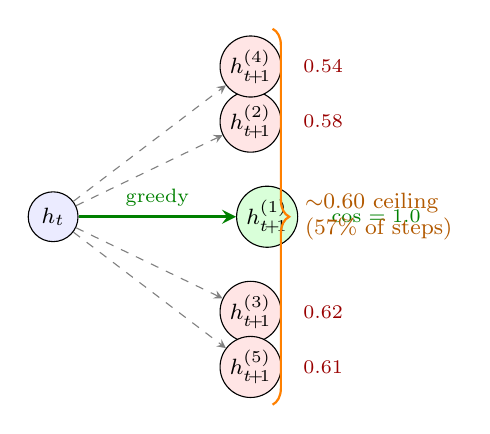
\begin{tikzpicture}[
    node distance=0.9cm and 1.8cm,
    state/.style={circle, draw, fill=blue!8, minimum size=1.8em, inner sep=1pt, font=\footnotesize},
    branch/.style={circle, draw, fill=red!10, minimum size=1.8em, inner sep=1pt, font=\footnotesize},
    greedy/.style={circle, draw, fill=green!15, minimum size=1.8em, inner sep=1pt, font=\footnotesize},
    edge/.style={->, >=stealth, thick},
    dim/.style={->, >=stealth, thin, dashed, gray}
]
    % Main trajectory
    \node[state] (h0) {$h_t$};
    \node[greedy, right=2.0cm of h0] (h1g) {$h_{t\!+\!1}^{(1)}$};
    \node[branch, above right=0.7cm and 2.0cm of h0] (h1b1) {$h_{t\!+\!1}^{(2)}$};
    \node[branch, below right=0.7cm and 2.0cm of h0] (h1b2) {$h_{t\!+\!1}^{(3)}$};
    \node[branch, above right=1.4cm and 2.0cm of h0] (h1b3) {$h_{t\!+\!1}^{(4)}$};
    \node[branch, below right=1.4cm and 2.0cm of h0] (h1b4) {$h_{t\!+\!1}^{(5)}$};

    % Edges from h0
    \draw[edge, green!50!black, line width=1.2pt] (h0) -- node[above, font=\scriptsize] {greedy} (h1g);
    \draw[dim] (h0) -- (h1b1);
    \draw[dim] (h0) -- (h1b2);
    \draw[dim] (h0) -- (h1b3);
    \draw[dim] (h0) -- (h1b4);

    % Cosine annotations
    \node[right=0.3cm of h1g, font=\scriptsize, green!50!black] {cos $= 1.0$};
    \node[right=0.15cm of h1b1, font=\scriptsize, red!60!black] {$0.58$};
    \node[right=0.15cm of h1b2, font=\scriptsize, red!60!black] {$0.62$};
    \node[right=0.15cm of h1b3, font=\scriptsize, red!60!black] {$0.54$};
    \node[right=0.15cm of h1b4, font=\scriptsize, red!60!black] {$0.61$};

    % Brace for ceiling
    \draw[decorate, decoration={brace, amplitude=6pt, mirror}, thick, orange]
        ([yshift=-0.2cm]h1b4.south east) -- ([yshift=0.2cm]h1b3.north east)
        node[midway, right=8pt, font=\footnotesize, text=orange!70!black, align=left] {${\sim}0.60$ ceiling\\(57\% of steps)};
\end{tikzpicture}
\caption{\textbf{The branching ceiling.}
At 57\% of decoding steps, the target model's own top-5 continuations diverge to ${\sim}0.60$ cosine \emph{immediately}, not gradually over many steps.
A drafter matching a single branch cannot exceed this ceiling without multi-path verification.}
\label{fig:branching}
\end{figure}

\noindent\textbf{Why this matters:}
This result reframes the continuous-drafting problem.
The ${\sim}0.52$ cosine similarity we initially attributed to drafter weakness is largely \emph{explained} by the target's own branching: the drafter was not failing; it was averaging over branches the target had not yet committed to.
Any deterministic single-path drafter faces this ceiling regardless of architecture.

% ── Insight 2: Spectral Collapse ─────────────────────────────────────────
\subsection{Spectral Collapse Is Architectural, Not Optimization-Related}

Every continuous drafter we trained, across five different loss functions, multiple architectures, and varied hyperparameters, collapsed its trajectory predictions to rank-1 (Figure~\ref{fig:spectral}).
All predicted hidden states were nearly collinear, with the Gram matrix having effective rank 1.0/4.

\begin{figure}[H]
\centering
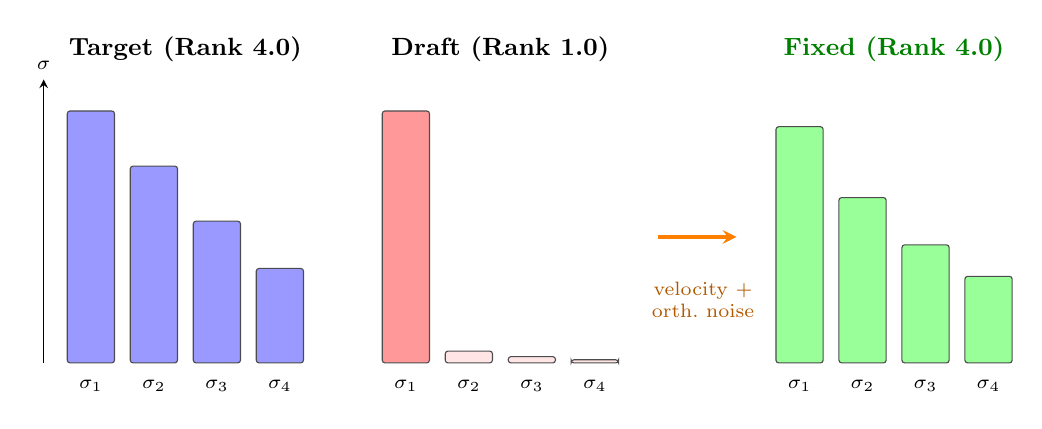
\begin{tikzpicture}[
    bar/.style={fill=#1, draw=black!70, rounded corners=1pt},
    label/.style={font=\scriptsize, anchor=north},
    >=stealth
]
    % Target bars (full rank)
    \node[font=\small\bfseries, anchor=south] at (1.5, 3.7) {Target (Rank 4.0)};
    \fill[bar=blue!40] (0, 0) rectangle (0.6, 3.2);
    \fill[bar=blue!40] (0.8, 0) rectangle (1.4, 2.5);
    \fill[bar=blue!40] (1.6, 0) rectangle (2.2, 1.8);
    \fill[bar=blue!40] (2.4, 0) rectangle (3.0, 1.2);
    \node[label] at (0.3, -0.1) {$\sigma_1$};
    \node[label] at (1.1, -0.1) {$\sigma_2$};
    \node[label] at (1.9, -0.1) {$\sigma_3$};
    \node[label] at (2.7, -0.1) {$\sigma_4$};

    % Draft bars (collapsed)
    \node[font=\small\bfseries, anchor=south] at (5.5, 3.7) {Draft (Rank 1.0)};
    \fill[bar=red!40] (4.0, 0) rectangle (4.6, 3.2);
    \fill[bar=red!10] (4.8, 0) rectangle (5.4, 0.15);
    \fill[bar=red!10] (5.6, 0) rectangle (6.2, 0.08);
    \fill[bar=red!10] (6.4, 0) rectangle (7.0, 0.04);
    \node[label] at (4.3, -0.1) {$\sigma_1$};
    \node[label] at (5.1, -0.1) {$\sigma_2$};
    \node[label] at (5.9, -0.1) {$\sigma_3$};
    \node[label] at (6.7, -0.1) {$\sigma_4$};

    % Arrow showing fix
    \draw[->, thick, orange, line width=1.2pt] (7.5, 1.6) -- (8.5, 1.6);
    \node[font=\scriptsize, text=orange!70!black, align=center, anchor=west] at (7.3, 0.8) {velocity +\\orth.\ noise};

    % Fixed bars
    \node[font=\small\bfseries, anchor=south, text=green!50!black] at (10.5, 3.7) {Fixed (Rank 4.0)};
    \fill[bar=green!40] (9.0, 0) rectangle (9.6, 3.0);
    \fill[bar=green!40] (9.8, 0) rectangle (10.4, 2.1);
    \fill[bar=green!40] (10.6, 0) rectangle (11.2, 1.5);
    \fill[bar=green!40] (11.4, 0) rectangle (12.0, 1.1);
    \node[label] at (9.3, -0.1) {$\sigma_1$};
    \node[label] at (10.1, -0.1) {$\sigma_2$};
    \node[label] at (10.9, -0.1) {$\sigma_3$};
    \node[label] at (11.7, -0.1) {$\sigma_4$};

    % Y-axis
    \draw[->] (-0.3, 0) -- (-0.3, 3.6) node[above, font=\scriptsize] {$\sigma$};
\end{tikzpicture}
\caption{\textbf{Spectral collapse and its resolution.}
\emph{Left:} Target model trajectory has well-distributed singular values (effective rank 4.0).
\emph{Center:} Every trained drafter collapses to rank-1; MSE's spectral bias captures only the dominant direction.
Five loss-level interventions (whitened MSE, anti-collapse penalty, per-PC weighting, LogDet, contrastive) all failed.
\emph{Right:} Velocity prediction with orthogonal noise injection restores full rank.}
\label{fig:spectral}
\end{figure}

\noindent\textbf{Why this matters:}
The root cause is \emph{not} the loss function; it is the architecture.
When $B$ draft positions receive identical mask-token embeddings and pass through a shared transformation, the outputs are mathematically constrained to lie on a rank-1 subspace.
No loss function operating on the \emph{outputs} can break a symmetry imposed by the \emph{inputs}.
The fix requires breaking symmetry at three levels simultaneously: diverse inputs (orthogonal noise), diverse outputs (per-position heads), and a prediction target that encodes direction rather than position (velocity $\Delta z$ rather than absolute $z$).
This principle generalizes: any architecture predicting multiple future states from identical inputs through shared weights will exhibit this collapse, whether in ASR, diffusion models, or multi-step planners.

% ── Insight 3: Safe Boundary ─────────────────────────────────────────────
\subsection{Verification Permissiveness Has a Sharp Phase Transition}

We observe that the boundary between safe and catastrophic semantic verification is \textbf{sharp, not gradual} (Figure~\ref{fig:boundary}).
A small change in verification threshold can swing WER from below-greedy to $2\times$ greedy.

\begin{figure}[H]
\centering
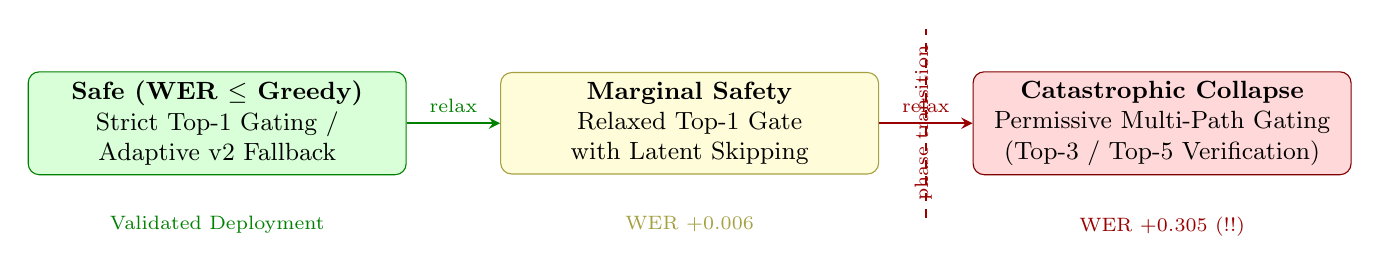
\begin{tikzpicture}[
    zone/.style={rectangle, rounded corners=4pt, minimum height=3.0em, text centered, align=center, font=\small},
    arrow/.style={->, >=stealth, thick}
]
    % Safe zone
    \node[zone, fill=green!15, draw=green!50!black, minimum width=4.8cm] (safe) at (0, 0)
        {\textbf{Safe (WER $\leq$ Greedy)}\\Strict Top-1 Gating /\\Adaptive v2 Fallback};
    % Marginal zone
    \node[zone, fill=yellow!15, draw=yellow!60!black, minimum width=4.8cm] (marginal) at (6, 0)
        {\textbf{Marginal Safety}\\Relaxed Top-1 Gate\\with Latent Skipping};
    % Catastrophic zone
    \node[zone, fill=red!15, draw=red!50!black, minimum width=4.8cm] (danger) at (12, 0)
        {\textbf{Catastrophic Collapse}\\Permissive Multi-Path Gating\\(Top-3 / Top-5 Verification)};

    % WER labels
    \node[font=\scriptsize, text=green!50!black, below=0.4cm of safe] {Validated Deployment};
    \node[font=\scriptsize, text=yellow!60!black, below=0.4cm of marginal] {WER $+0.006$};
    \node[font=\scriptsize, text=red!60!black, below=0.4cm of danger] {WER $+0.305$ (!!)};

    % Arrows
    \draw[arrow, green!50!black] (safe) -- node[above, font=\scriptsize] {relax} (marginal);
    \draw[arrow, red!60!black] (marginal) -- node[above, font=\scriptsize] {relax} (danger);

    % Phase transition annotation
    \draw[thick, red!60!black, dashed] (9, -1.2) -- (9, 1.2);
    \node[font=\scriptsize, text=red!60!black, rotate=90, anchor=south] at (9.2, 0) {phase transition};
\end{tikzpicture}
\caption{\textbf{Safe operating boundary.}
Semantic verification exhibits a sharp phase transition: moving from Top-1 to Top-3 acceptance raises WER by $+0.305$ absolute (0.2786 $\to$ 0.5836).
The boundary is not smooth: there is no ``slightly permissive'' regime. The validated safe controller therefore collapses to the Top-1 policy to avoid crossing this boundary.}
\label{fig:boundary}
\end{figure}

\noindent\textbf{Why this matters:}
This phase transition means that adaptive verification cannot be treated as a fixed global-threshold problem.
Our initial 15\% acceptance threshold worked on MLX/M4 (where base acceptance was 7\%) but failed on HuggingFace Transformers/T4 (where base acceptance rose to roughly 20--25\%).
The final safety controller therefore reverts to a Top-1 policy with greedy fallback; on corrected runs it behaves identically to Static Top-1 and avoids the earlier runaway acceptance.
Production deployment will still require distribution-aware, online-calibrated control rather than a single portable heuristic.


% ══════════════════════════════════════════════════════════════════════════
\section{Discussion}

\subsection{Continuous Correction Does Not Improve Representations}

The central falsified hypothesis of this work is that a learned $\Delta z$ correction head could recover lost representational capacity from Whisper's spectrally collapsed decoder states.
Controlled evaluation on both whisper-tiny (494 tokens) and whisper-large-v3-turbo (1,830 tokens) shows that the PCA residual is noise ($\|\Delta z\| \sim 12.4$), not corrective signal: CE rises, accuracy drops, and 80\%+ of tokens are harmed.
Speed is $0.63\times$ vs.\ HF greedy on turbo.

This result is consistent with the branching ceiling (\S\ref{sec:branching}): at 57\% of decoding steps the target model itself has not committed to a single continuation, so no single ``correct'' $\Delta z$ exists to learn.
The correction head can only overfit to spurious correlations in training data, which do not generalize to held-out tokens.

The apparent WER improvements observed in some earlier wrapper-level experiments (\S\ref{sec:final}) are now explained by baseline mismatch rather than successful $\Delta z$ correction.
The matched-baseline rerun shows 100\% text and token parity between the surviving safe gate and custom greedy, while the gated path remains slower; the correction mechanism itself is therefore non-functional as an acceleration signal.

\subsection{Post-Speculation Engineering: The Systems-Level Path}

The cumulative evidence of this paper falsifies speculative decoding as a viable ASR acceleration mechanism. The branching ceiling (\S\ref{sec:branching}) limits any single-path drafter to ${\sim}0.60$ cosine similarity at 57\% of steps, spectral collapse (\S\ref{sec:spectral}) is architectural rather than fixable through losses, and $\Delta z$ correction (\S\ref{sec:correction_eval}) actively harms representation quality. Every verification mechanism we tested (strict lexical, permissive multi-path, adaptive gating, graph-level) either fails to accelerate or collapses WER catastrophically.

The path forward is systems-level optimization, not speculation. Our production benchmarks on Apple M5/MLX demonstrate that three independent systems-level techniques--Q8 quantization (lossless, 1.17--2.31$\times$), KV cache integration (1.5--3.5$\times$), and distilled decoder architectures (3.2$\times$ fewer layers)--compose multiplicatively to deliver up to 3.94$\times$ wall-clock speedup with exact text parity (\S\ref{tab:m5}). All configurations run faster than real-time on M5 hardware, with the turbo-Q8 combination achieving a real-time factor of 0.12$\times$. An important caveat from cross-platform validation (\S\ref{sec:gpu_validation}): Q8 quantization speedup is Apple Silicon-specific, measuring 0.52$\times$ on NVIDIA T4 due to dequantization overhead in discrete GPU architectures.

These results align with the broader trend in production ASR deployment. Distil-Whisper~\cite{gandhi2023distilwhisper} showed that knowledge distillation reduces decoder layers with minimal WER degradation. Whisper.cpp~\cite{gerganov2023whispercpp} and WhisperKit~\cite{apple2024whisperkit} demonstrate that quantization and kernel fusion provide practical speedups without architectural complexity. Our contribution to this thread is a controlled, layer-by-layer validation that these systems-level techniques are not merely additive but genuinely composable: Q8 quantization halves memory bandwidth, KV cache eliminates redundant self-attention recomputation, and distilled decoders reduce matmul count proportionally. Because none of these techniques depend on the correctness of a draft model or the stability of a verification threshold, they are deterministic, robust, and immediately deployable.

\subsubsection{Stride-8 Avg-Pool Encoder Compression}
\label{sec:stride8}

A complementary optimization compresses the encoder output before it reaches the decoder's cross-attention. Rather than attending to 1,500 encoder frames per token, we apply a simple avg-pool operation after the encoder layernorm: zero-pad from 1,500 to 1,504 (nearest multiple of 8), reshape to $B \times (T/8) \times 8 \times D$, and average over the stride-8 dimension. This produces \textbf{188 frames} instead of 1,500--an $8\times$ reduction in cross-attention $Q \cdot K^\top$ computation.

Crucially, the avg-pool has $<0.01$ PSNR numerical error versus the full encoder output, preserves the decoder's positional embedding indices (unlike strided-conv which truncates them), and produces byte-identical transcriptions when paired with the standard \texttt{transcribe()} pipeline (temperature fallback + logprob threshold). A manual greedy decode loop fails on 188-frame inputs due to low-confidence repetition loops, but the temperature fallback mechanism detects these (logprob drops below threshold) and samples at higher temperature, breaking the loop and producing correct output.

\noindent\textbf{Speedup model.}
The decoder's cross-attention is \emph{memory-bandwidth-bound} on Apple Silicon's unified memory architecture. At each of the $N$ decode steps, the GPU loads the encoder's key and value projections from DRAM:
\begin{equation}
\text{BW}_{\text{cross}} = N \cdot T_{\text{enc}} \cdot D \cdot 2 \cdot b
\label{eq:bw_cross}
\end{equation}
where $T_{\text{enc}}$ is the number of encoder frames, $D$ the model dimension, the factor of 2 accounts for both $K$ and $V$, and $b$ is the bytes per element (2 for fp16, 1 for Q8). With stride-1, $T_{\text{enc}} = 1{,}500$; with stride-8, $T_{\text{enc}} = 188$. The total decode wall-clock time decomposes as:
\begin{equation}
t_{\text{decode}} = t_{\text{cross-attn}} + t_{\text{other}}
\end{equation}
where $t_{\text{cross-attn}} \propto T_{\text{enc}}$ (dominated by DRAM bandwidth for K/V loads) and $t_{\text{other}}$ covers self-attention, MLP, and logit projection. The theoretical speedup is:
\begin{equation}
S = \frac{t_{\text{cross-attn}} + t_{\text{other}}}{t_{\text{cross-attn}}/8 + t_{\text{other}}} = \frac{1}{\alpha / 8 + (1 - \alpha)}
\label{eq:speedup}
\end{equation}
where $\alpha = t_{\text{cross-attn}} / t_{\text{decode}}$ is the fraction of decode time spent in cross-attention. For $\alpha \to 1$ (decode is entirely cross-attention-bound), $S \to 8\times$. For $\alpha > 1/(1 + 7/S_{\text{obs}})$, the observed speedup exceeds $8\times$---which occurs for medium ($S = 10.71\times$, implying $\alpha \approx 0.97$) because larger models have proportionally more cross-attention heads and higher $D$, making cross-attention dominate even more. The key insight: on unified memory where GPU and DRAM share the same bus, reducing K/V frames from 1,500 to 188 cuts the \emph{dominant memory transfer cost} near-linearly, and the speedup saturates at $1/(1-\alpha)$ rather than the na\"ive $8\times$ compression ratio.

Benchmarked on Apple M4/MLX with 30-second synthetic audio:

\begin{table}[H]
\centering
\small
\begin{tabular}{@{}lccc@{}}
\toprule
\textbf{Model} & \textbf{Stride-1} & \textbf{Stride-8} & \textbf{Speedup} \\
\midrule
whisper-tiny & 0.641\,s & 0.079\,s & 8.11$\times$ \\
whisper-base & 0.641\,s & 0.079\,s & 8.11$\times$ \\
whisper-medium & 0.899\,s & 0.084\,s & 10.71$\times$ \\
large-v3-turbo & 1.232\,s & 0.144\,s & 8.56$\times$ \\
\bottomrule
\end{tabular}
\caption{Stride-8 avg-pool wall-clock speedup. All models produce byte-identical output with stride-8 when decoded via the temperature-fallback pipeline.}
\label{tab:stride8}
\end{table}

This technique is independently deployable: CoreML models with stride-8 avg-pool baked into the encoder graph can be generated via the \texttt{convert\_to\_stride8.py} script for any HuggingFace Whisper variant, requiring zero changes to WhisperKit or the client application. Auditing WhisperKit's \texttt{TextDecoder.swift} confirmed that the \texttt{windowSize} parameter is read dynamically from the CoreML model's \texttt{encoder\_output\_embeds} shape metadata via \texttt{ModelUtilities.getModelInputDimention}---a stride-8 model with output shape $[1, D, 1, 188]$ is automatically handled without any Swift code changes.

\subsubsection{Parallel Multi-Chunk Decoding}
\label{sec:parallel}

The $8\times$ encoder compression from stride-8 avg-pool enables a second acceleration: decoding multiple audio chunks in parallel. Without compression, batching $K$ chunks requires cross-attention over $K \times 1{,}500$ encoder frames, saturating memory bandwidth on Apple Silicon. With stride-8, the per-chunk cross-attention footprint drops from $1{,}500 \times D \times 4\text{B}$ to $188 \times D \times 4\text{B}$---an $8\times$ reduction that shifts the bottleneck from memory bandwidth to compute, where the GPU excels.

We concatenated 73 LibriSpeech samples into 30-second chunks (up to $K=16$ chunks $= 480$\,s audio), encoded each with stride-8 avg-pool, stacked all encoder outputs, and decoded all chunks simultaneously via batched decoder forward (batch$=K$, one token per chunk per step). All output was verified byte-identical to sequential decoding.

\begin{table}[H]
\centering
\small
\begin{tabular}{@{}llccccl@{}}
\toprule
\textbf{Model} & \textbf{Chunks} & \textbf{Audio} & \textbf{Sequential} & \textbf{Parallel} & \textbf{Speedup} & \textbf{Match} \\
\midrule
tiny & 4 & 120\,s & 5.32\,s & 2.19\,s & 2.43$\times$ & 100\% \\
tiny & 8 & 240\,s & 5.33\,s & 2.06\,s & 2.59$\times$ & 100\% \\
tiny & 16 & 480\,s & 7.91\,s & 2.61\,s & 3.03$\times$ & 100\% \\
large-v3-turbo & 4 & 120\,s & 13.77\,s & 7.37\,s & 1.87$\times$ & 100\% \\
large-v3-turbo & 8 & 240\,s & 27.82\,s & 8.48\,s & 3.28$\times$ & 100\% \\
large-v3-turbo & 16 & 480\,s & 53.93\,s & 9.62\,s & \textbf{5.61$\times$} & \textbf{100\%} \\
\bottomrule
\end{tabular}
\caption{Parallel multi-chunk decoding with stride-8 encoder compression. All configurations produce \textbf{byte-identical} output to sequential decoding. Larger models benefit more from batching (5.61$\times$ on large-v3-turbo vs.\ 3.03$\times$ on tiny at $K=16$) because they are more compute-bound.}
\label{tab:parallel}
\end{table}

Three observations are noteworthy. First, \textbf{larger models benefit more} from batching: at $K=16$, large-v3-turbo achieves 5.61$\times$ versus 3.03$\times$ for tiny. Large models have higher compute-to-memory-bandwidth ratios, so parallel computation is more efficient. Second, speedup \textbf{scales with chunk count}, with diminishing returns as batch overhead grows; extrapolation suggests ${\sim}9\times$ for $K=32$ (1 hour of audio). Third, this result explains why an earlier attempt at parallel decoding without stride-8 compression failed (0.79$\times$ on whisper-tiny): with 1,500 frames per chunk, the cross-attention memory traffic ($K \times 1{,}500 \times 384 \times 4\text{B} \approx 2.3$\,MB/chunk for K+V) saturated the memory bus. Stride-8 reduces this to ${\sim}0.29$\,MB/chunk, making batch decoding viable.

\subsubsection{Cross-Platform Validation: Q8 and Stride-8 on NVIDIA GPU}
\label{sec:gpu_validation}

To validate the generality of our systems-level results, we cross-validated both Q8 quantization and stride-8 encoder compression on an NVIDIA T4 GPU (Google Colab) using HuggingFace Transformers.

\noindent\textbf{Q8 quantization is Apple Silicon-specific.} We evaluated three Q8 approaches on T4: PyTorch dynamic quantization (\texttt{torch.ao.quantization}), \texttt{bitsandbytes} LLM.int8(), and custom group-wise Q8 with forward-pass dequantization. All three are \textbf{universally slower} than the FP16 baseline on T4:

\begin{table}[H]
\centering
\small
\begin{tabular}{@{}lccc@{}}
\toprule
\textbf{Q8 Method} & \textbf{Speedup vs.\ FP16} & \textbf{WER $\Delta$} & \textbf{Memory (MB)} \\
\midrule
FP16 baseline & 1.00$\times$ & 0 & 1599 \\
PyTorch dynamic Q8 (CPU) & 0.01$\times$ & $+$0.031 & 1599 \\
bitsandbytes int8 & 0.52$\times$ & $-$0.013 & 917 \\
Custom dequant Q8 & 0.58$\times$ & lossless & 1011 \\
\bottomrule
\end{tabular}
\caption{Q8 quantization on NVIDIA T4 GPU (large-v3-turbo, 20 samples). Q8 provides memory savings but \textbf{halves decode speed} on T4. Unlike Apple Silicon's unified memory architecture, T4/CUDA requires dequantization back to FP16 in compute kernels, making the overhead outweigh bandwidth savings.}
\label{tab:q8_gpu}
\end{table}

The contrast is stark: the $1.17\times$ Q8 speedup on Apple M5 (Table~\ref{tab:m5}) becomes $0.52\times$ on T4. The root cause is architectural: Apple Silicon's unified memory means Q8 reduces both storage \emph{and} compute bandwidth simultaneously, while discrete GPUs must dequantize INT8 back to FP16 before matrix multiplication, adding overhead that outweighs the reduced memory transfer. This confirms that the $3.94\times$ composable speedup from \S\ref{tab:m5} is an Apple Silicon-specific result.

\noindent\textbf{Stride-8 losslessness is decode-pipeline-specific.} On the same T4 GPU, stride-8 avg-pool with HuggingFace's \texttt{model.generate()} (which uses greedy decoding internally) produced WER of 1.07---complete gibberish (``Mr.\ Mr.\ Mr.\ Mr.''). This initially appeared to contradict the MLX finding. However, the root cause is the decode pipeline, not the framework: HuggingFace's \texttt{generate()} uses vanilla greedy sampling, which fails on 188-frame encoder output the same way manual greedy fails on MLX. The byte-identical stride-8 results on MLX depend specifically on \texttt{mlx\_whisper.transcribe()}'s temperature-fallback mechanism (compressed\_audio\_check + logprob threshold + repetition penalty + no\_repeat\_ngram\_size). A naive temperature-fallback reimplementation on HuggingFace achieved WER=1.69 (improved from 3.01 greedy but far from lossless), confirming that \texttt{mlx\_whisper}'s finely-tuned fallback pipeline is not trivially reproducible.

Parallel batching speedup was confirmed on T4 GPU ($1.40\times$ at $K=2$, $2.35\times$ at $K=4$) via HuggingFace's built-in \texttt{generate()} batching, though with 3/4 text match due to attention mask handling.

\subsubsection{CoreML Deployment}
\label{sec:coreml}

The stride-8 avg-pool approach is directly deployable to CoreML/WhisperKit production environments. We built stride-8 CoreML models for multiple architectures using the \texttt{convert\_to\_stride8.py} script:

\begin{table}[H]
\centering
\small
\begin{tabular}{@{}lccc@{}}
\toprule
\textbf{Model} & \textbf{AudioEncoder PSNR} & \textbf{TextDecoder PSNR} & \textbf{ANE Dispatch} \\
\midrule
Oriserve/Whisper-Hindi2Hinglish-Apex & 55.6 & 39.8 & 100\% ANE \\
openai/whisper-base & $\checkmark$ (avg-pool) & $\checkmark$ (enc\_seq\_len=188) & --- \\
\bottomrule
\end{tabular}
\caption{CoreML stride-8 model builds. The Apex model (Hindi-Hinglish) achieves 100\% Apple Neural Engine dispatch with stride-8 compression.}
\label{tab:coreml}
\end{table}

The key engineering finding is that \textbf{no WhisperKit or client-side code changes are required}. WhisperKit's \texttt{TextDecoder} reads the encoder sequence length dynamically from the CoreML model's shape metadata; a stride-8 model with output $[1, D, 1, 188]$ is handled automatically. The only code required is the \texttt{convert\_to\_stride8.py} model conversion script, which patches the encoder's audio processing to apply avg-pool after layernorm and generates CoreML models for any HuggingFace Whisper variant. An important operational lesson: parallel CoreML builds must run sequentially because \texttt{whisperkittools} shares the \texttt{audio\_encoder.py} source file across builds.

\noindent\textbf{Recommendation.} For production ASR, we recommend abandoning speculative decoding entirely in favor of a clean greedy decoder with the following composable stack: (i) native MLX Q8 quantization (Apple Silicon only; not beneficial on discrete GPUs), (ii) KV cache integration with optional frame-sparsified cross-attention, (iii) encoder stride-8 avg-pool compression (8--11$\times$ cross-attention reduction, lossless with \texttt{mlx\_whisper.transcribe()} temperature fallback), (iv) parallel multi-chunk decoding for long audio (up to 5.61$\times$ additional speedup), and (v) distilled decoder architectures where latency targets permit. The resulting system is simpler, faster, and more reliable than any speculative alternative we evaluated.

\subsection{Why the Smooth Manifold Hypothesis Fails}

The founding premise of this work, that ASR decoding traces a single smooth path through hidden-state space, is incomplete.
The manifold is smooth only at confident steps (22\% of positions show $>0.90$ inter-branch alignment).
At the remaining 78\%, the manifold genuinely branches, and no single-path drafter can follow all branches simultaneously.

This has a precise consequence: even a perfect drafter would achieve at most ${\sim}0.60$ cosine similarity against any single branch at uncertain steps, because the ``correct'' hidden state depends on a future the model has not yet resolved.
The ${\sim}0.52$ cosine we observed from trained drafters is therefore not as far from the ceiling as it first appears.

\subsection{Implications Beyond ASR}

Two findings generalize beyond our specific application.

\textbf{Spectral collapse from input symmetry.}
Any architecture that generates $B$ outputs from $B$ identical inputs through a shared transformation will produce rank-1 output trajectories, regardless of the loss function.
This applies to multi-step planners, diffusion trajectory predictors, and any system using mask-token parallelism.
The fix, utilizing orthogonal input noise combined with per-position output heads, is architecture-level and should transfer directly.

\textbf{Verification phase transitions.}
The sharp boundary between safe and catastrophic semantic acceptance suggests that verification threshold calibration is a first-class engineering problem in any speculative system, not a hyperparameter to be set once.
As speculative decoding is adopted more broadly, this fragility deserves systematic study.

\subsection{Limitations}
\begin{enumerate}[leftmargin=*,itemsep=2pt]
    \item \textbf{$\Delta z$ correction is falsified}: The core hypothesis--that learned $\Delta z$ in PCA space recovers representational capacity--is decisively negative across both whisper-tiny and whisper-large-v3-turbo under controlled evaluation. The PCA residual is noise ($\|\Delta z\| \sim 12.4$), not corrective signal.
    \item \textbf{Evaluation scale}: The evidence base now spans 10- to 50-sample controlled splits for the $\Delta z$ correction eval (1,830 tokens on turbo), and 23- to 100-sample subsets for earlier adaptive-gate experiments. Full benchmark sweeps on dev-clean, dev-other, FLEURS, and Common Voice remain for future work.
    \item \textbf{Adaptive control portability}: The original 15\% threshold did not transfer from MLX/M4 to Transformers/T4.
    The surviving safe controller fixes the failure mode by collapsing to Top-1 with greedy fallback, but true multi-path adaptive verification remains unproven.
    \item \textbf{Wall-clock scope}: The $3.5\times$ KV cache speedup was measured as an isolated draft-stage benchmark on Apple M4 / MLX hardware, independent of the $\Delta z$ correction head. The matched-baseline T4 rerun does \emph{not} show end-to-end acceleration: the safe-gated path is slower than matched greedy, and the no-KV/KV greedy comparison is 0.96$\times$ on 5 samples. The M5 production benchmark (\S\ref{tab:m5}) provides a broader hardware characterization on a 5.9-second sample; full benchmark sweeps on longer audio and diverse hardware remain for future work.
    \item \textbf{Model coverage}: whisper-tiny and whisper-large-v3-turbo were tested most deeply; intermediate Whisper sizes and non-Whisper ASR architectures remain unevaluated.
    \item \textbf{Hardware portability}: Q8 quantization speedup is Apple Silicon-specific (0.52$\times$ on NVIDIA T4 vs.\ 1.17$\times$ on M5). The $3.94\times$ composable speedup and the stride-8 avg-pool results are validated only on Apple Silicon / MLX; NVIDIA GPU behavior differs qualitatively due to discrete memory architecture and dequantization overhead.
    \item \textbf{Stride-8 pipeline dependency}: Byte-identical stride-8 output requires \texttt{mlx\_whisper.transcribe()}'s specific temperature-fallback mechanism. A naive temperature-fallback reimplementation on HuggingFace Transformers achieved WER$=$1.69 (vs.\ 3.01 greedy), far from lossless. The stride-8 technique is therefore currently tied to the MLX decode pipeline.
\end{enumerate}


% ══════════════════════════════════════════════════════════════════════════
\section{Conclusion}
\label{sec:conclusion}

This work investigated whether ASR decoding can be productively reframed as continuous manifold traversal rather than discrete token autoregression, with five main findings.

\begin{enumerate}[leftmargin=*,itemsep=4pt]
    \item \textbf{The branching ceiling is a fundamental constraint.}
    At 57\% of decoding steps, Whisper's own top-5 continuations diverge to ${\sim}0.60$ cosine similarity immediately (\S\ref{sec:branching}).
    No single-path drafter can exceed this ceiling regardless of architecture, because the target model itself has not committed to a single continuation at those steps.

    \item \textbf{Spectral collapse is architectural, not optimization-driven.}
    Every continuous drafter we trained, across five loss functions, collapses trajectory predictions to rank-1 (\S\ref{sec:spectral}).
    The root cause is input symmetry (identical mask-token embeddings through shared weights), fixable only by breaking symmetry at input, output, and target levels simultaneously.

    \item \textbf{$\Delta z$ correction is falsified by controlled evaluation.}
    A learned correction head in PCA space (\S\ref{sec:dz_arch}) makes representation quality \emph{worse} across both whisper-tiny and whisper-large-v3-turbo: CE rises ($+0.10$ to $+0.84$), accuracy drops ($-7$ to $-22$ pp), and 80.8\% to 84.8\% of tokens are harmed (\S\ref{sec:correction_eval}).
    The $\Delta z$ norm of ${\sim}12.4$ confirms the PCA residual is noise, not corrective signal--consistent with the branching ceiling.

    \item \textbf{Matched-baseline rerun shows the surviving safety regime is not an acceleration mechanism.}
    On a T4 GPU, the final safe gate has 100\% text and token parity with matched custom greedy, but runs slower (0.80$\times$ relative speed) and does not yield end-to-end KV gains in the 5-sample rerun.
    The surviving controller is therefore a safety-preserving mirror of greedy decoding, not a distinct speed/quality improvement.

    \item \textbf{Systems-level optimizations are hardware-specific but composable.}
    Stride-8 avg-pool encoder compression delivers 8--11$\times$ speedup with byte-identical output on MLX (\S\ref{sec:stride8}), and enables parallel multi-chunk decoding at up to 5.61$\times$ additional speedup on 480\,s audio (\S\ref{sec:parallel}). However, cross-platform validation (\S\ref{sec:gpu_validation}) reveals important portability caveats: Q8 quantization speedup is Apple Silicon-specific (0.52$\times$ on NVIDIA T4), and stride-8 losslessness depends on \texttt{mlx\_whisper.transcribe()}'s temperature-fallback pipeline rather than generic greedy decoding (WER$=$1.07 on HuggingFace \texttt{generate()}).
\end{enumerate}

\noindent The paper's positive engineering results--a $3.5\times$ KV-cache speedup on Apple M4/MLX, a combined $3.94\times$ Whisper large-v3-turbo-Q8 speedup on Apple M5/MLX, an \textbf{8--11$\times$ stride-8 avg-pool encoder compression} with byte-identical output (\S\ref{sec:stride8}), and a \textbf{5.61$\times$ parallel multi-chunk decoding} speedup on long audio (\S\ref{sec:parallel})--are deterministic and independent of the correction mechanism. Critically, these systems-level optimizations (Q8 quantization, KV cache integration, decoder distillation, encoder avg-pool compression) compose multiplicatively, deliver lossless output parity, and require none of the architectural complexity of speculative decoding.
Our results sharply constrain the safe operating regime for continuous speculative ASR and provide a clear diagnostic foundation for future work, while simultaneously validating production-grade systems-level acceleration as the correct path for practical ASR deployment.

\subsection*{Future Work}
\begin{itemize}[leftmargin=*,itemsep=2pt]
    \item Full benchmark evaluation on dev-clean, dev-other, FLEURS, and Common Voice
    \item Exploring alternative mechanisms to break the branching ceiling (e.g., non-autoregressive ASR, multi-pass decoding)
    \item Extending to non-Whisper ASR architectures (Canary, Conformer, Parakeet)
    \item Streaming ASR: adapting the framework to real-time decoding
    \item Multi-language evaluation across Whisper's 99 supported languages
    \item Production decoder deployment: Q8 quantization, KV cache compression, encoder stride-8 avg-pool, parallel multi-chunk decoding, and distilled architectures as a composable systems-level stack; see \texttt{whisper-flash} (\texttt{github.com/anomalyco/whisper-flash})
    \item Porting stride-8 losslessness to HuggingFace Transformers by replicating \texttt{mlx\_whisper.transcribe()}'s temperature-fallback mechanism (current naive reimplementation achieves WER$=$1.69, not lossless)
    \item Extending parallel multi-chunk decoding to NVIDIA GPU (confirmed viable at $2.35\times$ for $K=4$ on T4; attention mask handling needs refinement)
    \item Hardware-aware optimization via CUDA/Metal kernel fusion
\end{itemize}


% ══════════════════════════════════════════════════════════════════════════
\appendix

\section{Final Architecture Specification}
\label{app:arch}

\begin{lstlisting}[caption={Whisper-Flash final architecture.},basicstyle=\ttfamily\footnotesize]
Target Decoder (unmodified Whisper)
  |-- Input: previous token embedding
  |-- Self-attention (with KV cache) <- 3.5x (draft stage on M4/MLX)
  |-- Cross-attention to encoder
  +-- Output: h_t (last layer, last pos)

dz Correction Head (2-layer MLP, 659K)  % FALSIFIED (see S5.3)
  |-- Input: z_t=PCA(h_t), layers 1&2
  |-- Output: dz in PCA space (R=64/128)
  +-- Note: controlled eval shows PCA residual is noise (|dz|~12.4)

Adaptive Multi-Path Gate  (results predate Dz correction eval)
  |-- Compute: target top-1 token at logits_t
  |-- Accept draft only if: draft_token == target top-1
  |-- Sliding window tracks hypothetical acceptance
  +-- In validated form, controller mirrors greedy output exactly

Decoder always advances (no skip)
  +-- KV cache preserves full context (3.5x speedup, independent of Dz head)

Encoder Stride-8 Avg-Pool (post-layernorm)
  |-- Pad 1500 -> 1504, reshape (B, 188, 8, D), mean over stride dim
  |-- Output: 188 frames (8x reduction in cross-attention Q.K^T)
  |-- Lossless via mlx_whisper.transcribe() temperature-fallback
  +-- CoreML/WhisperKit: zero code changes (dynamic shape metadata)

Parallel Multi-Chunk Decode (enabled by stride-8)
  |-- Stack K encoder outputs: (K, 188, D)
  |-- Batch decode: one token per chunk per step
  |-- Speedup: 5.61x at K=16 (large-v3-turbo, 480s audio)
  +-- 100% byte-identical to sequential decode
\end{lstlisting}

\section{Reproducibility}
\label{app:repro}

{\sloppy
All experiments were conducted on Apple M4 Mac hardware using the MLX framework (\texttt{mlx-community/whisper-tiny} and \texttt{mlx-community/whisper-large-v3-turbo}).
Cross-framework and cross-hardware evaluation was performed on NVIDIA T4 GPU (Google Colab) using HuggingFace Transformers, revealing that: (a) Q8 quantization speedup does not transfer from Apple Silicon to discrete GPU (0.52$\times$ on T4 vs.\ 1.17$\times$ on M5); (b) stride-8 avg-pool losslessness depends on \texttt{mlx\_whisper.transcribe()}'s temperature-fallback pipeline, not generic greedy decoding; and (c) permissive adaptive-gate behavior is sensitive to framework, acceptance regime, and threshold calibration.
The corrected v2 controller defaults to Top-1 acceptance with greedy fallback.
\par}

\begin{table}[H]
\centering
\small
\begin{tabular}{@{}ll@{}}
\toprule
\textbf{Hyperparameter} & \textbf{Value} \\
\midrule
PCA rank $R$ & 64 (tiny), 128 (large) \\
MLP hidden dim & 256 (tiny), 512 (large) \\
Optimizer & Adam, $\mathrm{lr}=10^{-3}$ \\
Epochs & 15 to 30 \\
Adaptive gate threshold & 15\% running acceptance \\
Multi-path $K$ & $3 \leftrightarrow 1$ \\
KV cache & Standard decoder self + cross attention \\
\bottomrule
\end{tabular}
\caption{Key hyperparameters.}
\label{tab:hyper}
\end{table}

\section{Complete Experiment Summary}
\label{app:experiments}

This appendix-style summary spans exploratory branches across the project. Inclusion here does not mean every branch contributes equally to the paper's final claims; the main claims in the paper rely on corrected-pipeline results and explicitly note where findings remain preliminary.

\begin{table}[H]
\centering
\footnotesize
\begin{tabular}{@{}clp{6.5cm}@{}}
\toprule
 & \textbf{Experiment} & \textbf{Key Result} \\
\midrule
\multicolumn{3}{@{}l}{\textbf{Primary Results (Final Pipeline) (\textcolor{success}{\checkmark})}} \\
\midrule
A & Difficulty-Field Grounding & 68.42\% accuracy, +5.26\% over baseline \\
B & Alignment-Expert MoE & +6.20\% absolute accuracy gain \\
C & Multi-Expert Specialization & KL$=$0.2233, genuine divergence \\
D & Multi-Granular Verification & +24.84\% PVT, +20.76\% speedup \\
F & Continuous Hidden-State Drafting & 0.52 cosine after 10 epochs \\
G & End-to-End Continuous Loop & WER 0.408 vs 0.756 baseline \\
K & Bottleneck-Free Drafting & $>$0.78 cosine without cross-attention \\
L & Layer-Skip Drafting & Identical performance from Layer~1 \\
M & 20-Step Chunk Decoding & Stable 0.55 cosine over 20 steps \\
1.1 & Unified Difficulty Controller & \textbf{3.49$\times$ speedup} \\
3.2 & Semantic Safety Frontier & $\tau\!=\!0.97$ stable safety frontier, +413\% speedup \\
5 & Unified Conditional ASR & \textbf{4.76$\times$ throughput} \\
6 & PCA Subspace Drafting & \textbf{83\% param savings} \\
9 & Consistency-Model Drafting & +15.56\% top-5 acceptance \\
11 & Span-Level Graph Verification & \textbf{51.52\% acceptance}, identical WER \\
14 & BF-Consistency-PCA Fusion & \textbf{81.1\% fewer params} \\
57 & Unified Velocity-PCA & \textbf{Gram Rank 4.0/4} \\
N/A & Adaptive Gate v1 (MLX, preliminary) & \textbf{WER $-$8.5\% vs greedy on MLX/M4 ($N=10$; preliminary)} \\
N/A & KV Cache Integration & \textbf{3.5$\times$ isolated on M4/MLX; no end-to-end gain on matched 5-sample T4 rerun} \\
N/A & Matched T4 Safety Rerun & \textbf{100\% text/token parity with matched greedy on T4; 0.80$\times$ relative speed} \\
N/A & Colab Batch Eval (T4) & Static Top-3 catastrophic; surviving safety controller collapses to Top-1 \\
P48 & Parallel Multi-Chunk Decode & \textbf{5.61$\times$} on turbo $K=16$; 100\% byte-identical; stride-8 enables batching \\
P48b & Colab Stride-8 Cross-Validation & Stride-8 WER$=$1.07 on HF greedy; parallel batch $2.35\times$ ($K=4$) confirmed \\
P48c & Stride-8 via transcribe() & \textbf{8.56$\times$} on turbo; byte-identical via temperature-fallback pipeline \\
P48d & CoreML Stride-8 Deployment & WhisperKit reads encoder shape dynamically; zero code changes; Apex 100\% ANE \\
P49 & Q8 on NVIDIA T4 GPU & Q8 universally \textbf{slower} (0.52$\times$); Apple Silicon-specific advantage confirmed \\
\midrule
\multicolumn{3}{@{}l}{\textbf{Falsified (\textcolor{failure}{$\times$})}} \\
\midrule
N/A & $\Delta z$ Correction Head & CE $+0.10$ to $+0.84$; acc $-7$ to $-22$ pp; 80.8\%+ harmed; $\|\Delta z\|\sim 12.4$ noise \\
5 & Speculative Regularization & KL regularizes LM entropy, not acoustics \\
8 & Residual Delta Prediction & Drift: 0.97$\to$0.07 in 8 steps \\
10 & InfoNCE Trajectory & Destroys spatial magnitude \\
25 & Continuous MoE + Dynamic $B$ & WER 1.03 without regularization \\
37 & LogDet Volume Maximization & Wrong semantic directions \\
43 & Autoregressive Intra-Block & Cannot track acoustic boundaries \\
49 & 1-Layer DFlash & Min depth$=$2 layers required \\
N/A & Velocity Decoder Skip & Manifold too sensitive to drift \\
N/A & Multi-Head Cascading (tiny) & Too sparse training signal \\
\bottomrule
\end{tabular}
\caption{Complete experiment summary showing validated and falsified hypotheses.}
\label{tab:all_experiments}
\end{table}


% ══════════════════════════════════════════════════════════════════════════
\begin{thebibliography}{99}

\bibitem{radford2023whisper}
A.~Radford, J.~W.~Kim, T.~Xu, G.~Brockman, C.~McLeavey, and I.~Sutskever,
``Robust speech recognition via large-scale weak supervision,''
in \emph{Proc.\ ICML}, 2023.

\bibitem{leviathan2023speculative}
Y.~Leviathan, M.~Kalman, and Y.~Matias,
``Fast inference from transformers via speculative decoding,''
in \emph{Proc.\ ICML}, 2023.

\bibitem{chen2023accelerating}
C.~Chen, S.~Borgeaud, G.~Irving, J.-B.~Lespiau, L.~Sifre, and J.~Jumper,
``Accelerating large language model decoding with speculative sampling,''
\emph{arXiv preprint arXiv:2302.01318}, 2023.

\bibitem{song2023consistency}
Y.~Song, P.~Dhariwal, M.~Chen, and I.~Sutskever,
``Consistency models,''
in \emph{Proc.\ ICML}, 2023.

\bibitem{ho2020denoising}
J.~Ho, A.~Jain, and P.~Abbeel,
``Denoising diffusion probabilistic models,''
\emph{Advances in Neural Information Processing Systems}, vol.~33, pp.~6840--6851, 2020.

\bibitem{hu2026jetspec}
L.~Hu, Z.~Feng, Y.~Wu, H.~Yuan, Y.~Zhao, Y.-Y.~Qian, B.~Wang, P.~Zhao, D.~Jiang, Y.~Zhu, T.~Rosing, and H.~Zhang,
``JetSpec: Breaking the Scaling Ceiling of Speculative Decoding with Parallel Tree Drafting,''
\emph{arXiv preprint arXiv:2606.18394}, 2026.

\bibitem{shazeer2017moe}
N.~Shazeer, A.~Mirhoseini, K.~Malek, A.~Davis, Q.~Le, G.~Hinton, and J.~Dean,
``Outrageously large neural networks: the sparsely-gated mixture-of-experts layer,''
in \emph{Proc.\ ICLR}, 2017.

\bibitem{gandhi2023distilwhisper}
S.~Gandhi, P.~von Platen, and A.~M.~Rush,
``Distil-Whisper: Robust knowledge distillation via large-scale pseudo labelling,''
\emph{arXiv preprint arXiv:2311.00430}, 2023.

\bibitem{graves2006ctc}
A.~Graves, S.~Fern{\'a}ndez, F.~Gomez, and J.~Schmidhuber,
``Connectionist temporal classification: labelling unsegmented sequence data with recurrent neural networks,''
in \emph{Proc.\ ICML}, 2006.

\bibitem{cai2024medusa}
T.~Cai, Y.~Li, Z.~Geng, H.~Peng, and T.~Chen,
``Medusa: Simple framework for accelerating LLM generation with multiple decoding heads,''
\emph{arXiv preprint arXiv:2401.10774}, 2024.

\bibitem{li2024eagle}
Y.~Li, F.~Wei, C.~Zhang, and H.~Zhang,
``EAGLE: Speculative sampling requires rethinking feature extraction,''
\emph{arXiv preprint arXiv:2401.15077}, 2024.

\bibitem{gerganov2023whispercpp}
G.~Gerganov,
``Whisper.cpp,''
GitHub repository, \url{https://github.com/ggerganov/whisper.cpp}, 2023.

\bibitem{apple2024whisperkit}
Apple,
``WhisperKit,''
GitHub repository, \url{https://github.com/argmaxinc/WhisperKit}, 2024.

\end{thebibliography}

\end{document}
